		\documentclass[a4paper,12pt,brazil]{book}

% tentei incluir o da pasta comum mas não funcionou
% \usepackage{amssymb}                        %%% para simbolo de 'marca registrada'
\usepackage[brazil]{varioref}               %%% referencias com página \vref
\usepackage[sf,bf,compact,topmarks,calcwidth,pagestyles]{titlesec} %%% definir títulos de seção
\usepackage{amsmath,amsfonts,amstext,amsthm,textcomp}
\usepackage{fancybox}                       %%% boxes
\usepackage[dvipsnames,usenames]{color}                          %%% Cores de fonte e fundo
\usepackage[dvipsnames,usenames]{xcolor}
\usepackage{colortbl}                       %%% Cores em tabelas
\usepackage{rotating}
\usepackage{fancyvrb}                       %%% Inclusão de texto usando VerbatimInput
\usepackage{bookman}                        %%% Fonte de Letras
\usepackage{enumerate}
\usepackage{lettrine}
\usepackage{minted}	
\usepackage{caption}
\usepackage{framed}
\usepackage{enumitem}

%\usepackage{listings}
%\lstset{
%  numbers=left,
%  numberstyle=\tiny,
%  mathescape=true,
%  frame=single,
%  stepnumber=1,
%%  basicstyle=\scriptsize, % fontes menores nos codigos
%  keywordstyle=\ttfamily,
%  identifierstyle=\ttfamily, % \bfseries negrito nos codigos
%  commentstyle=\ttfamily
%}
\usepackage{pstricks} % listings color: black!50!red

\usepackage{listings}
\lstset{
	numbers=left,
	stepnumber=1,
	firstnumber=1,
	numberstyle=\tiny,
	mathescape=true,
	extendedchars=true,
	breaklines=true,
	frame=single,
	basicstyle=\footnotesize,
%	basicstyle=\scriptsize,
	stringstyle=\ttfamily,
% 	moredelim=*[l][\itshape]{||},%
	showstringspaces=false,
	float=h,
}
\lstdefinelanguage{lalp} {
  sensitive=true,
  keywordstyle={\color{black!50!green}\ttfamily\bfseries},
  keywords={const, typedef, fixed, in, out, counter, when, block_ram, delay_op, mult_op_s, add_reg_op_s},
  otherkeywords={<-},
  otherkeywords={@},
  commentstyle={\color{black!50!red}\itshape},
  morecomment=[l]{//}, 
  morecomment=[s]{/*}{*/},
}
\lstdefinelanguage{ican} {
  sensitive=true,
  keywordstyle={\color{black!50!red}\ttfamily\bfseries},
  keywords={array, begin, boolean, by, case, character, default, do, each, elif, else, end, enum, esac, false, fi, for, goto, if, in, inout, integer, nil, od, of, out, procedure, real, record, repeat, return, returns, sequence, set, to, true, until, where, while},
  commentstyle={\color{black!50!green}\itshape},
  morecomment=[l]{||},
  literate={{(X)}{$\times$}1 {(E)}{$\in$}1 {(U)}{$\cup$}1 {(N)}{$\cap$}1 {(<)}{$\langle$}1 {(>)}{$\rangle$}1 {->}{$\rightarrow$}2 {<\-}{$\leftarrow$}2 {=}{$=$}1 {>}{$>$}1 {<}{$<$}1 {!=}{$\neq$}1 {>=}{$\ge$}1 {<=}{$\le$}1}
}

\renewcommand\listingscaption{Algoritmo}
\renewcommand\listoflistingscaption{Lista de Algoritmos}


\usepackage[english,brazil]{babel}
\usepackage[utf8]{inputenc}
\usepackage[T1]{fontenc}
\usepackage{times}
\usepackage{graphicx,xr}
\usepackage{subfigure}
\usepackage{longtable}
\usepackage{setspace}
\usepackage{multirow}
\usepackage{rotating}
\usepackage{indentfirst}
\usepackage{xspace}
\usepackage[sort]{natbib}
\usepackage[a4paper,top=30mm,bottom=20mm,left=30mm,right=20mm]{geometry}

\usepackage{hyperref}
\hypersetup{
%  backref, %omitir na versão final
  pdfsubject =	{...},
  pdftitle =	{...},
  pdfkeywords = {...},
  pdfauthor =	{Ricardo Menotti, Daniel Lucrédio, ...},
  colorlinks =	{true}, %true na versão final
  linkcolor =	{black!50!blue},
  citecolor =	{black!50!blue},
  urlcolor =	{black!50!blue},
}

\exhyphenpenalty = 10000

\onehalfspace

\hyphenation{es-ta-be-le-ci-das a-tu-al-men-te Simple-Scalar-ARM}

\newcommand{\up}[1]{\raisebox{1.5ex}[0pt]{#1}}

\newcommand{\bi}{\begin{itemize}}
\newcommand{\ei}{\end{itemize}}
\newcommand{\be}{\begin{enumerate}}
\newcommand{\ee}{\end{enumerate}}

\definecolor{Gray}{gray}{0.9}

% using \autoref{} instead
%\newcommand{\reffig}[1]{Figura~\ref{fig:#1}}
%\newcommand{\reftab}[1]{Tabela~\ref{tab:#1}}
%\newcommand{\refcha}[1]{Capítulo~\ref{cha:#1}}
%\newcommand{\refses}[1]{Seção~\ref{ses:#1}}
%\newcommand{\refsub}[1]{Subseção~\ref{sub:#1}}
%\newcommand{\refape}[1]{Apêndice~\ref{ape:#1}}
%\newcommand{\refcod}[1]{Código~\ref{cod:#1}}
\newcommand{\subfigureautorefname}{\figureautorefname}

\newcommand{\cha}[2]{\chapter{#2}\label{cha:#1}} %\thispagestyle{empty}
\newcommand{\ses}[2]{\section{#2}\label{ses:#1}}
\newcommand{\sub}[2]{\subsection{#2}\label{sub:#1}}
\newcommand{\ape}[2]{\chapter{#2}\label{ape:#1}} %\thispagestyle{empty}

\newcommand{\figsim}[2]{
\begin{figure}[!ht]
  \centering
  \includegraphics[width=\textwidth]{../figuras/#1.jpg}
  \caption{#2}
  \label{fig:#1}
\end{figure}
}

\newcommand{\ew}[1]{\selectlanguage{english}\emph{#1}\selectlanguage{brazil}}
%\newcommand{\ew}[1]{\emph{#1}}

\renewcommand{\bibname}{Referências Bibliográficas}

\setcounter{secnumdepth}{2}

\setcounter{tocdepth}{2}

\pagestyle{empty}

%\font\numberfont= goxi2074 scaled 2000      %%% Fonte para o Número do Capítulo
\font\numberfont= pzcmi scaled 6500      %%% Fonte para o Número do Capítulo

                                            %%% redefine o formato do título
\titleformat{\chapter}[display]
  {\normalfont\Large\sffamily
  }
  {
   \rule[32pt]{.7\linewidth}{4pt}
   \hspace{-10pt}
   \shadowbox{
   \begin{minipage}{.18\linewidth}
     \begin{center}
       \textsc{\Large\chaptertitlename}\\
       \vspace{1ex}
       {\numberfont \thechapter}\\
       \vspace{1ex}
     \end{center}
   \end{minipage}}
  }
  {0pt}
  {\filcenter
   \Huge
   }
  [\hfill\rule{.8\textwidth}{0.75pt}\\
     \vskip-1.8ex\hfill\rule{.7\textwidth}{2pt}]


\newpagestyle{body}{ %[\small\sffamily]{
\headrule

\sethead[\thepage][][\ifthechapter{\thechapter\quad}{} \textsl{\chaptertitle}]%
          {\ifthechapter{\thechapter\quad \textsl{\chaptertitle}}{\textsl{\chaptertitle}}}{}{\thepage}


}

\newpagestyle{misc}{
  \headrule
  \sethead{\textsl{\chaptertitle}}{}{\thepage}
  \setfoot{}{}{}
}

\font\largefont= pzcmi scaled 6500

\newcommand{\versal}[1]{{\noindent
    \setbox0\hbox{\largefont #1 }%
    \count0=\ht0                   % height of versal
    \count1=\baselineskip          % baselineskip
    \divide\count0 by \count1      % versal height/baselineskip
    \dimen1 = \count0\baselineskip % distance to drop versal
    \advance\count0 by 1\relax     % no of indented lines
    \dimen0=\wd0                   % width of versal
    \global\hangindent\dimen0      % set indentation distance
    \global\hangafter-\count0      % set no of indented lines
    \hskip-\dimen0\setbox0\hbox to\dimen0{\raise-\dimen1\box0\hss}%
    \dp0=0in\ht0=0in\box0}}


%%%  define linha mais grossa para tabelas

\newdimen\arrayruleHwidth
\setlength{\arrayruleHwidth}{2pt} \makeatletter
\def\Hline{\noalign{\ifnum0=`}\fi\hrule \@height \arrayruleHwidth
\futurelet \@tempa\@xhline} \makeatother

\definecolor{mygreen}{rgb}{0.1, 0.6, 0.2}

\usepackage{amssymb}                        %%% para simbolo de 'marca registrada'
\usepackage[brazil]{varioref}               %%% referencias com página \vref
\usepackage[sf,bf,compact,topmarks,calcwidth,pagestyles]{titlesec} %%% definir títulos de seção
\usepackage{amsmath,amsfonts,amstext,amsthm,textcomp}
\usepackage{fancybox}                       %%% boxes
\usepackage[dvipsnames,usenames]{color}                          %%% Cores de fonte e fundo
\usepackage[dvipsnames,usenames]{xcolor}
\usepackage{colortbl}                       %%% Cores em tabelas
\usepackage{rotating}
\usepackage{fancyvrb}                       %%% Inclusão de texto usando VerbatimInput
\usepackage{bookman}                        %%% Fonte de Letras
\usepackage{enumerate}
\usepackage{lettrine}
\usepackage{minted}	
\usepackage{caption}
\usepackage{framed}
\usepackage{enumitem}

%\usepackage{listings}
%\lstset{
%  numbers=left,
%  numberstyle=\tiny,
%  mathescape=true,
%  frame=single,
%  stepnumber=1,
%%  basicstyle=\scriptsize, % fontes menores nos codigos
%  keywordstyle=\ttfamily,
%  identifierstyle=\ttfamily, % \bfseries negrito nos codigos
%  commentstyle=\ttfamily
%}
\usepackage{pstricks} % listings color: black!50!red

\usepackage{listings}
\lstset{
	numbers=left,
	stepnumber=1,
	firstnumber=1,
	numberstyle=\tiny,
	mathescape=true,
	extendedchars=true,
	breaklines=true,
	frame=single,
	basicstyle=\footnotesize,
%	basicstyle=\scriptsize,
	stringstyle=\ttfamily,
% 	moredelim=*[l][\itshape]{||},%
	showstringspaces=false,
	float=h,
}
\lstdefinelanguage{lalp} {
  sensitive=true,
  keywordstyle={\color{black!50!green}\ttfamily\bfseries},
  keywords={const, typedef, fixed, in, out, counter, when, block_ram, delay_op, mult_op_s, add_reg_op_s},
  otherkeywords={<-},
  otherkeywords={@},
  commentstyle={\color{black!50!red}\itshape},
  morecomment=[l]{//}, 
  morecomment=[s]{/*}{*/},
}
\lstdefinelanguage{ican} {
  sensitive=true,
  keywordstyle={\color{black!50!red}\ttfamily\bfseries},
  keywords={array, begin, boolean, by, case, character, default, do, each, elif, else, end, enum, esac, false, fi, for, goto, if, in, inout, integer, nil, od, of, out, procedure, real, record, repeat, return, returns, sequence, set, to, true, until, where, while},
  commentstyle={\color{black!50!green}\itshape},
  morecomment=[l]{||},
  literate={{(X)}{$\times$}1 {(E)}{$\in$}1 {(U)}{$\cup$}1 {(N)}{$\cap$}1 {(<)}{$\langle$}1 {(>)}{$\rangle$}1 {->}{$\rightarrow$}2 {<\-}{$\leftarrow$}2 {=}{$=$}1 {>}{$>$}1 {<}{$<$}1 {!=}{$\neq$}1 {>=}{$\ge$}1 {<=}{$\le$}1}
}

\renewcommand\listingscaption{Algoritmo}
\renewcommand\listoflistingscaption{Lista de Algoritmos}


\usepackage[english,brazil]{babel}
\usepackage[utf8]{inputenc}
\usepackage[T1]{fontenc}
\usepackage{times}
\usepackage{graphicx,xr}
\usepackage{subfigure}
\usepackage{longtable}
\usepackage{setspace}
\usepackage{multirow}
\usepackage{rotating}
\usepackage{indentfirst}
\usepackage{xspace}
\usepackage[sort]{natbib}
\usepackage[a4paper,top=30mm,bottom=20mm,left=30mm,right=20mm]{geometry}

\usepackage{hyperref}
\hypersetup{
%  backref, %omitir na versão final
  pdfsubject =	{...},
  pdftitle =	{...},
  pdfkeywords = {...},
  pdfauthor =	{Ricardo Menotti, Daniel Lucrédio, ...},
  colorlinks =	{true}, %true na versão final
  linkcolor =	{black!50!blue},
  citecolor =	{black!50!blue},
  urlcolor =	{black!50!blue},
}

\exhyphenpenalty = 10000

\onehalfspace

\hyphenation{es-ta-be-le-ci-das a-tu-al-men-te Simple-Scalar-ARM}

\newcommand{\up}[1]{\raisebox{1.5ex}[0pt]{#1}}

\newcommand{\bi}{\begin{itemize}}
\newcommand{\ei}{\end{itemize}}
\newcommand{\be}{\begin{enumerate}}
\newcommand{\ee}{\end{enumerate}}

\definecolor{Gray}{gray}{0.9}

% using \autoref{} instead
%\newcommand{\reffig}[1]{Figura~\ref{fig:#1}}
%\newcommand{\reftab}[1]{Tabela~\ref{tab:#1}}
%\newcommand{\refcha}[1]{Capítulo~\ref{cha:#1}}
%\newcommand{\refses}[1]{Seção~\ref{ses:#1}}
%\newcommand{\refsub}[1]{Subseção~\ref{sub:#1}}
%\newcommand{\refape}[1]{Apêndice~\ref{ape:#1}}
%\newcommand{\refcod}[1]{Código~\ref{cod:#1}}
\newcommand{\subfigureautorefname}{\figureautorefname}

\newcommand{\cha}[2]{\chapter{#2}\label{cha:#1}} %\thispagestyle{empty}
\newcommand{\ses}[2]{\section{#2}\label{ses:#1}}
\newcommand{\sub}[2]{\subsection{#2}\label{sub:#1}}
\newcommand{\ape}[2]{\chapter{#2}\label{ape:#1}} %\thispagestyle{empty}

\newcommand{\figsim}[2]{
\begin{figure}[!ht]
  \centering
  \includegraphics[width=\textwidth]{../figuras/#1.jpg}
  \caption{#2}
  \label{fig:#1}
\end{figure}
}

\newcommand{\ew}[1]{\selectlanguage{english}\emph{#1}\selectlanguage{brazil}}
%\newcommand{\ew}[1]{\emph{#1}}

\renewcommand{\bibname}{Referências Bibliográficas}

\setcounter{secnumdepth}{2}

\setcounter{tocdepth}{2}

\pagestyle{empty}

%\font\numberfont= goxi2074 scaled 2000      %%% Fonte para o Número do Capítulo
\font\numberfont= pzcmi scaled 6500      %%% Fonte para o Número do Capítulo

                                            %%% redefine o formato do título
\titleformat{\chapter}[display]
  {\normalfont\Large\sffamily
  }
  {
   \rule[32pt]{.7\linewidth}{4pt}
   \hspace{-10pt}
   \shadowbox{
   \begin{minipage}{.18\linewidth}
     \begin{center}
       \textsc{\Large\chaptertitlename}\\
       \vspace{1ex}
       {\numberfont \thechapter}\\
       \vspace{1ex}
     \end{center}
   \end{minipage}}
  }
  {0pt}
  {\filcenter
   \Huge
   }
  [\hfill\rule{.8\textwidth}{0.75pt}\\
     \vskip-1.8ex\hfill\rule{.7\textwidth}{2pt}]


\newpagestyle{body}{ %[\small\sffamily]{
\headrule

\sethead[\thepage][][\ifthechapter{\thechapter\quad}{} \textsl{\chaptertitle}]%
          {\ifthechapter{\thechapter\quad \textsl{\chaptertitle}}{\textsl{\chaptertitle}}}{}{\thepage}


}

\newpagestyle{misc}{
  \headrule
  \sethead{\textsl{\chaptertitle}}{}{\thepage}
  \setfoot{}{}{}
}

\font\largefont= pzcmi scaled 6500

\newcommand{\versal}[1]{{\noindent
    \setbox0\hbox{\largefont #1 }%
    \count0=\ht0                   % height of versal
    \count1=\baselineskip          % baselineskip
    \divide\count0 by \count1      % versal height/baselineskip
    \dimen1 = \count0\baselineskip % distance to drop versal
    \advance\count0 by 1\relax     % no of indented lines
    \dimen0=\wd0                   % width of versal
    \global\hangindent\dimen0      % set indentation distance
    \global\hangafter-\count0      % set no of indented lines
    \hskip-\dimen0\setbox0\hbox to\dimen0{\raise-\dimen1\box0\hss}%
    \dp0=0in\ht0=0in\box0}}


%%%  define linha mais grossa para tabelas

\newdimen\arrayruleHwidth
\setlength{\arrayruleHwidth}{2pt} \makeatletter
\def\Hline{\noalign{\ifnum0=`}\fi\hrule \@height \arrayruleHwidth
\futurelet \@tempa\@xhline} \makeatother

\definecolor{mygreen}{rgb}{0.1, 0.6, 0.2}


\title{Título}

\begin{document}
\selectlanguage{brazil}

%!TEX root = ios.tex

\begin{center}
%\normalfont\sffamily

\begin{minipage}[c]{\textwidth}
  \parbox[c]{3cm}{
      \begin{flushright}
      
\includegraphics[width=.25\textwidth]{../figuras/LogoUfscar}
      \end{flushright}
  }
  \parbox[c]{12cm}
    {
      \begin{center}
      \textbf{\Large Universidade Federal de São Carlos}

      \vspace{0.07cm}

      \textbf{\large Centro de Ciências Exatas e de Tecnologia}

      \vspace{0.07cm}

      \textbf{\large Departamento de Computação}
      \vspace{0.07cm}
      \end{center}
    }
\end{minipage}

\vspace{-0.5cm}
\rule{7.5cm}{0.03pc}{\tiny $_\diamondsuit$}\rule{7.5cm}{0.03pc}

\vspace*{20ex}

\textbf{\Large {Introdução às tecnologias para desenvolvimento de \\ aplicações em plataformas móveis iOS}} \\
\large{ Processo: \textbf{23112.003595/2012-35}}

\vspace*{5ex}

{\Large{ Coordenadores:  }} \\
\textbf{\Large{ Ricardo Menotti}} \\
\textbf{\Large{ Daniel Lucrédio}}

\vspace*{5ex}

{\Large{ Autor/Bolsista:  }}  \\
\textbf{\Large{ Régis Magno Zangirolami } } 
%\textbf{\Large{ Matheus Fernando Finatti }}  \\

\vspace*{10ex}

\textbf{\large São Carlos - SP, \today}

\vspace*{5ex}


\includegraphics[width=.25\textwidth]{../figuras/LogoDC} \hfill

\includegraphics[width=.25\textwidth]{../figuras/LogoProEx}

\end{center} 

\pagestyle{empty}

\clearpage

\selectlanguage{brazil}
\onehalfspace

\pagestyle{plain}
\pagenumbering{roman}

\setcounter{tocdepth}{1} % 0 capítulos, 1 seções, 2 subseções
\tableofcontents
\clearpage % se o verso ficar em branco...% VAI
\thispagestyle{empty}

\listoffigures
\addcontentsline{toc}{section}{Lista de Figuras}
\clearpage % se o verso ficar em branco...% VAI
\thispagestyle{empty}

\listoftables
\addcontentsline{toc}{section}{Lista de Tabelas}
\clearpage % se o verso ficar em branco...% VAI
\thispagestyle{empty}

\listoflistings
\addcontentsline{toc}{section}{Lista de Algoritmos}
\clearpage % se o verso ficar em branco...% VAI
\thispagestyle{empty}

\chapter*{Lista de Abreviaturas}
\addcontentsline{toc}{section}{Lista de Abreviaturas}
\begin{longtable}{ll}
\end{longtable}

\usemintedstyle{perldoc}


\chapter*{Resumo}
\addcontentsline{toc}{section}{Resumo}

\begin{singlespace}
Esse material didático oferece uma visão geral de como programar para o sistema móvel Android e utilizar suas APIs nativas na criação de aplicativos. O material tentará cobrir desde o básico, como a configuração do ambiente de desenvolvimento, criação de layouts básicos e complexos, estrutura geral de um aplicativo e ir até a programação de aplicativos mais complexos que tentam utilizar uma ou várias APIs em conjunto.

O objetivo é dar apenas uma noção de como utilizar as ferramentas do Android, introduzir ao aluno os conceitos e não entrar em detalhes do sistema operacional ou em conceitos mais aprofundados, mas sim uma visão genérica.
Após a leitura desse material e realização da prática o aluno deve estar preparado para construir seus próprios aplicativos nativos, e poderá até monetizar seus aplicativos se desejar.
\end{singlespace}

\clearpage % se o verso ficar em branco...
\thispagestyle{empty}

\thispagestyle{empty}

\doublespace
%\onehalfspace
%\singlespace

\clearpage

\pagestyle{body}
\pagenumbering{arabic}

%%%%%%%%%%%%%%%%%%%%%%%%%%%%%%%%%%%%%%%%%%%%%%%%%%%%%%%%%%%%%%%%%%%%%%%%%%%%%%%%
\cha{introducao}{Introdução}
%\setcounter{page}{1}
%7-10p
O Android hoje está em centenas de milhões de dispositivos móveis ao redor do mundo, e vem crescendo. É uma plataforma para desenvolvimento em dispositivos móveis como \emph{smartphones}, \emph{tablets} e outros. 

Construído em uma colaboração \emph{open-source} com a comunidade de Linux, o Android se tornou a plataforma móvel mais utilizada e que mais cresce no mundo. Sua abertura o tornou o favorito de consumidores e desenvolvedores, levando a um rápido crescimento no número de aplicativos e jogos. Está disponível em centenas de dispositivos diferentes e de fabricantes diferentes em versões diferentes.

Atualmente\footnote{Data em que foi escrito: 06/2013} existem 4 principais versões do Android, são elas da mais atual para mais antiga:
\bi
\item \emph{Jelly Bean} versão 4.2 e 4.1 que trouxe otimizações de performance, uma nova interface do sistema e outros
\footnote{\emph{Jelly Bean}: \href{http://developer.android.com/about/versions/jelly-bean.html}{http://developer.android.com/about/versions/jelly-bean.html}}
\item \emph{Ice Cream Sandwich} versão 4.0 trouxe uma interface refinada e unificada para \emph{smartphones} e \emph{tablets} além de facilidade com multitasking e outros
\footnote{\emph{Ice Cream Sandwich}: \href{http://developer.android.com/about/versions/android-4.0-highlights.html}{http://developer.android.com/about/versions/android-4.0-highlights.html}}
\item \emph{Honeycomb} versão 3.0 desenvolvida exclusivamente para \emph{tablets}
\footnote{\emph{Honeycomb}: \href{http://developer.android.com/about/versions/android-3.0-highlights.html}{http://developer.android.com/about/versions/android-3.0-highlights.html}}
\item \emph{Gingerbread} versão 2.3 introduziu refinamentos da interface, mais performance e tornou o sistema mais intuitivo
\footnote{\emph{Gingerbread}: \href{http://developer.android.com/about/versions/android-2.3-highlights.html}{http://developer.android.com/about/versions/android-2.3-highlights.html}}
\ei

O Google coletou os dados referentes a distribuição das versões do Android:
\begin{table}[H]
\centering
    \begin{tabular}{|l|l|l|l|}
     \rowcolor{Gray} \hline 
    Versão        & Codinome           & API & Distribuição \\ \hline
    1.6           & Donut              & 4   & 0.1\%        \\ \hline
    2.1           & Eclair             & 7   & 1.5\%        \\ \hline
    2.2           & Froyo              & 8   & 3.2\%        \\ \hline
    2.3 - 2.3.2   & Gingerbread        & 9   & 0.1\%        \\ \hline
    2.3.3 - 2.3.7 & Gingerbread        & 10  & 36.4\%       \\ \hline
    3.2           & Honeycomb          & 13  & 0.1\%        \\ \hline
    4.0.3 - 4.0.4 & Ice Cream Sandwich & 15  & 25.6\%       \\ \hline
    4.1.x         & Jelly Bean         & 16  & 29.0\%       \\ \hline
    4.2.x         & Jelly Bean         & 17  & 4.0\%        \\ \hline
    \end{tabular}
    % REITRADO DE: http://developer.android.com/about/dashboards/index.html
    \caption{Tabela com as distribuições das versões do Android, todas as versões com menos de 0.1\% de participação foram desconsideradas}
\end{table}

\begin{figure}[H]
  \centering
  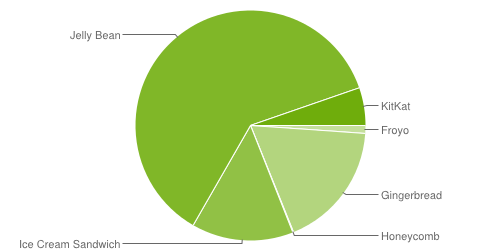
\includegraphics[width=.85\textwidth]{figuras/chart.png}
  \caption{Distribuição das versões do Android}
  \label{fig:d}
\end{figure}

\newpage
Esse material irá cobrir alguns tópicos no desenvolvimento de aplicativos para android, tais como:
\bi
\item
Configuracão do ambiente de desenvolvimento: Como configurar o ambiente para começar a desenvolver aplicativos, os primeiros passos para criar seu primeiro aplicativo de maneira simples;
\item
Elementos da interface: Como projetar seu aplicativo para usar as principais interfaces. Listas, Listas compostas, Grades, Abas, Menus são as interfaces mais usadas nos diversos aplicativos no mercado; e
\item
Elementos de hardware: Como projetar seu aplicativo para usar as APIs de hardware: Bluetooth, GPS, SMS, Chamadas.
\ei

 Para esse material, algumas convenções serão seguidas: 
 \bi
 \item
Os códigos estarão sempre com a sintaxe colorida para facilitar a leitura;
\item
URLs das referências estarão nas notas de rodapé; e
\item
 Dicas estarão envoltas por uma caixa para facilitar a visualização
\ei

% http://tug.ctan.org/tex-archive/macros/latex/contrib/minted/
% http://pygments.org/

\cha{configambiente}{Configuração do Ambiente}
A instalação e configuração do ambiente de desenvolvimento para Android é simples, o Google fornece um pacote chamado ADT \emph{(Android Development Tools)} que contém o ambiente Eclipse com o \emph{plugin} do Android, algumas ferramentas para instalação dos aplicativos nos \emph{smartphones}, o gerenciador do SDK e as imagens para o emulador do Android. Essas ferramentas são suficientes para o desenvolvimento na plataforma.
O pacote ADT pode ser encontrado em: \href{http://developer.android.com/sdk/}{Android SDK}\footnote{\href{http://developer.android.com/sdk/}{http://developer.android.com/sdk/}}. 

Basta fazer o download do pacote e extrair que tudo já está pré-configurado para iniciar o desenvolvimento, portanto não há muito o que configurar.

Caso opte por utilizar uma instalação já existente do ambiente Eclipse, você pode instalar o plugin do Android automaticamente através da ferramenta de instalação de plugins do ambiente. Após a instalação será necessário abrir o \emph{SDK Manager} e instalar:
\begin{itemize}[noitemsep, nolistsep]
\item \emph{Android SDK Tools};
\item \emph{Android SDK Platform-Tools}; e
\item Para cada API que você irá utilizar, instalar o \emph{SDK Platform} e opcionalmente o \emph{Documentation for Android SDK} e o \emph{Samples for SDK}.
\end{itemize}

\cha{intro-android}{Linguagem do Android}
\section{Linguagem}
A linguagem usada para programar na plataforma Android é Java. Então antes de engajar no aprendizado Android é altamente recomendável estudar material Java e principalmente o paradigma de orientação a objetos.

O Android tem algumas particulariedades na organização e configuração que é feita através de arquivos XML específicos do Android. Alguns arquivos XML servem para configurar o aplicativo, layout de cada tela e outros dão suporte a strings para facilitar o suporte a múltiplos idiomas.
Felizmente o conjunto Eclipse com ADT já cuida disso automaticamente e possui uma serie de facilidades alcançadas por meio de interfaces gráficas para os programadores. Por esse motivo, para qualquer iniciante nessa área e recomendável a utilizacão do ambiente Eclipse.

A criação de layouts dos aplicativos pode ser feita inteiramente através da interface gráfica disponível no ambiente, no estilo \textit{drag and drop}. 

\section{Entendendo a estrutura de uma aplicação Android}

Uma aplicação Android consiste de uma ou mais \emph{activities}. Uma \emph{activity} é uma tela com \emph{views} que interagem com o usuário. Como o Android segue o padrão MVC \emph{(Model-View-Control)} as \emph{activities} são os \emph{controllers} e as \emph{views}, \emph{views}. As \emph{activities} são classes do Java, o \emph{layout} e outros recursos são definidos em arquivos XML.

Dentre os diversos arquivos XML existentes na configuração de um aplicativo Android o mais importante é o \texttt{{AndroidManifest.xml}}
\footnote{Documentação do \texttt{AndroidManifest}: \href{The AndroidManifest.xml File}{http://developer.android.com/guide/topics/manifest/manifest-intro.html}}
 pois é nele que se exprimem as configurações gerais do aplicativo. Nesse texto não iremos adentrar muito nos detalhes das configurações, mas apenas deixar claro que é nesse arquivo que se colocam as versões do Android que seu aplicativo será compatível com, as permissões para usar os recursos do aparelho como Internet, GPS, Bluetooth, etc. 
 
 A pasta \texttt{src/} contém o pacote com as classes do seu aplicativo isto é, o código fonte do seu aplicativo. Tanto \emph{activites} como classes de suporte devem estar dentro do pacote.

Dentro da pasta \texttt{res/} de recursos, encontram-se outros arquivos, referentes à disposição do layout, valores de strings e imagens que sua aplicação irá utilizar. A pasta \texttt{layout/} junto com as pastas \texttt{drawable-*/} servem para dispor o layout. Cada \textit{drawable} comporta imagens para um tamanho diferente de tela, enquanto que a pasta de \textit{layout} contém a dispoção geral do layout. São nesses arquivos que se colocam os itens \emph{(views)} que irão nas telas, como botões, caixas de texto, caixas de seleção, etc.

Na pasta \texttt{values/} o mais importante é o arquivo \texttt{strings.xml} que contém os valores das strings do aplicativo. Sempre que você quiser referenciar alguma string, a mesma deverá estar expressa nesse arquivo. Fica fácil dessa forma fazer o aplicativo suportar múltiplos idiomas, pois basta traduzir esse único arquivo para alterar todos os textos do aplicativo.

A pasta \texttt{menu/} contém os \emph{layouts} do menus do aplicativo, esses são aqueles que podem ser acessados através da \emph{Action Bar}\footnote{\emph{ActionBar}: \href{http://developer.android.com/design/patterns/actionbar.html}{http://developer.android.com/design/patterns/actionbar.html}} ou através dos botões físicos do aparelho.

\newpage
\textbf{Resumindo:}
\begin{itemize}[noitemsep, nolistsep]
\item \texttt{AndroidManifest.xml}: Configurações gerais do aplicativo;
\item \texttt{src/}: Classes do aplicativo; e
\item \texttt{res/}: Recursos do aplicativo tais que:
	\begin{itemize}[nolistsep, noitemsep]
		\item \texttt{strings/}: Todos os textos da sua aplicação, suporte a múltiplos idiomas;	
		\item \texttt{layout/}: Todos os \emph{layouts} de suas telas \emph{(activites)};
		\item \texttt{drawable/}: Todas as imagens, separados por tamanho de tela; e
		\item \texttt{menu/}: \emph{layout} dos menus do aplicativo.
	\end{itemize}
\end{itemize}


%% FIRST APP %%
\cha{primeiro-aplicativo}{Criando seu primeiro aplicativo}
Para exemplificar a criação de um aplicativo, seguiremos o exemplo dado pelo próprio manual do Google sobre o Android 
(Ver original\footnote{Original em: \href{http://developer.android.com/training/basics/firstapp/creating-project.html}{http://developer.android.com/training/basics/firstapp/creating-project.html}}). 
Trata-se de aplicativo simples do tipo \emph{''Hello World''}.

Iniciaremos criando um novo projeto no Eclipse acessando o menu: \emph{File -> New -> Android Application Project}.

Na janela que apareceu você deve colocar o nome do aplicativo, do projeto e do pacote. O nome do pacote deve seguir a convenção do Java\footnote{Convenção sobre nome dos pacotes: \href{http://docs.oracle.com/javase/tutorial/java/package/namingpkgs.html}{http://docs.oracle.com/javase/tutorial/java/package/namingpkgs.html}}.
\begin{itemize}[noitemsep]
	\item \textit{Minimum Required SDK:} É a versão mínima do sistema operacional Android que sua aplicação irá suportar, o mais comum é a versão 8 do SDK que se refere ao Android 2.2. Alguns tipos de layouts mais complexos não são suportados em versões mais antigas;
	\item \textit{Target SDK:} É a versão principal do Android para qual seu aplicativo está sendo desenvolvido;
	\item \textit{Compile With:} Versão do Android com qual seu aplicativo será compilado; e
	\item \textit{Theme:} Cores do layout.
\end{itemize}


\begin{figure}[H]
  \centering
  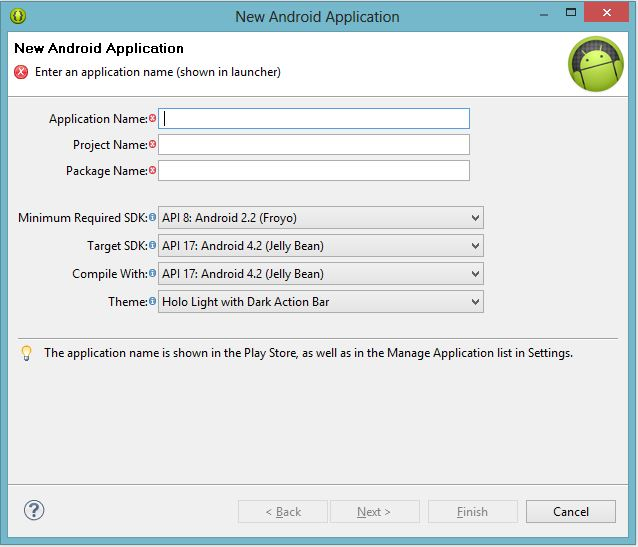
\includegraphics[width=.8\textwidth]{figuras/1-criando-app.jpg}
  \caption{Primeira janela de criação de novo aplicativo}
  \label{fig:d}
  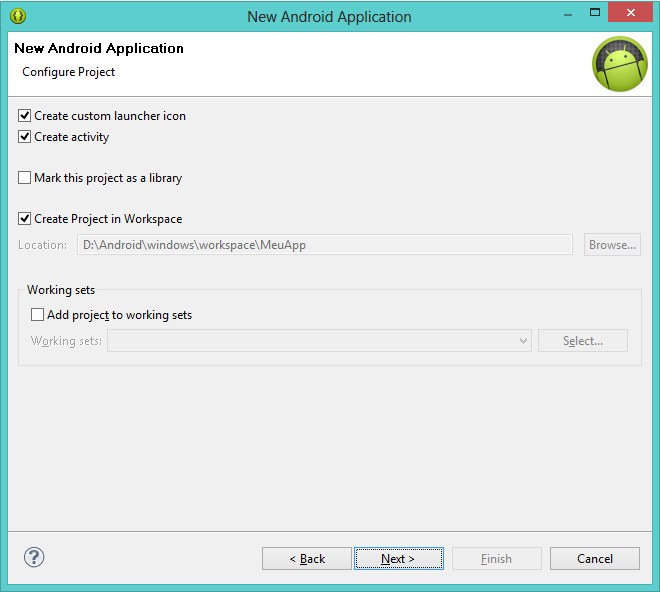
\includegraphics[width=.8\textwidth]{figuras/2-criando-app-2.png}
  \caption{Segunda janela de criação de novo aplicativo}
  \label{fig:c}
\end{figure}
\newpage
\begin{figure}[H]
  \centering
  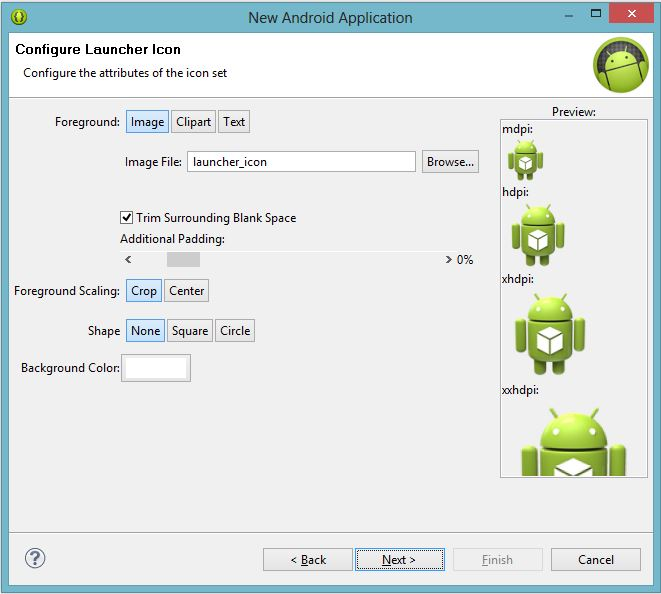
\includegraphics[width=.8\textwidth]{figuras/2-criando-app.jpg}
  \caption{Terceira janela de criação de novo aplicativo}
  \label{fig:c}
   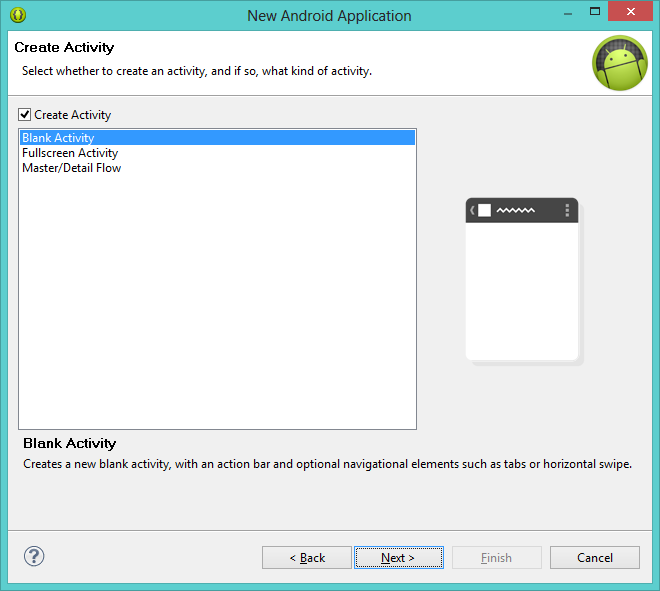
\includegraphics[width=.8\textwidth]{figuras/2-criando-app-4.png}
  \caption{Quarta janela de criação de novo aplicativo}
  \label{fig:c}
 \end{figure}
 \newpage
\begin{figure}[H]
  \centering
   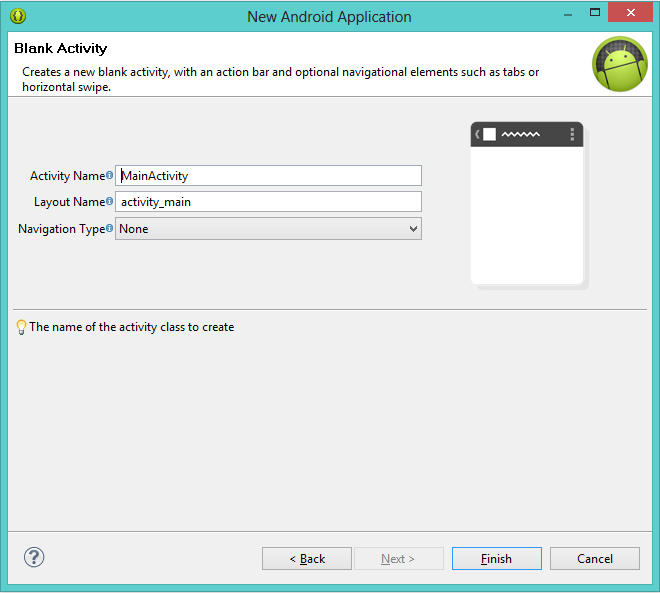
\includegraphics[width=.8\textwidth]{figuras/2-criando-app-5.png}
  \caption{Quinta janela de criação de novo aplicativo}
  \label{fig:c}
\end{figure}
\newpage
Observe na Figura 4.1 a janela de criação de uma nova aplicação Android. Em \emph{Application Name} você deve colocar o nome do aplicativo, em \emph{Project Name}, o nome do projeto e em \emph{Package Name} o nome do pacote. Para esse exemplo utilizaremos como \emph{Minimum Required SDK} a versão API 8, já que nesse exemplo não usaremos nenhum layout que não é suportado em versões mais antigas. Em \emph{Target SDK} e \emph{Compile With} optaremos pela versão mais nova, a API 17. Por final o \emph{Theme} eu optei pelo \emph{Holo Light with Dark Action Bar} que é um tema com fundo branco e barra superior preta, um dos padrões do Android.

\begin{framed}
\textbf{Dica:} Para obter o máximo de compatibilidade sempre procure utilizar \emph{layouts} compatíveis com versões antigas, observe na figura 1.1 que versões antigas ainda tem uma fatia considerável do mercado.
\end{framed}

A figura 4.2 mostra a segunda janela da configuração inicial do seu aplicativo. Você pode escolher um ícone personalizado se marcar a caixa \emph{Create custom launcher icon} o que te levará para a janela da figura 4.3. Se marcar \emph{Create Activity}  o assistente de criação te levará para a janela da figura 4.4 onde poderá escolher qual \emph{activity} vai ser criada para seu aplicativo. Em todos os exemplos escolheremos a opção \emph{Blank Activity}. Como nosso projeto não e uma biblioteca não marcaremos \emph{Mark this project as a library}. Se marcar \emph{Create Project in Workspace} o assistente irá salvar o projeto na pasta que foi configurada para o \emph{Workspace}, caso contrário ele irá pedir para escolher outro caminho. Como não trabalharemos com \emph{Working Sets} do Eclipse, a opção \emph{Add project to working sets} permanece desmarcada. 

Finalmente a figura 4.5 mostra a janela para nomear a \emph{activity} inicial, nesse exemplo mantive \emph{MainActivity}. O nome do \emph{layout} dessa \emph{activity} mantive como \emph{activity\_main} que é o padrão. Na caixa \emph{Navigation Type} existem algumas opções de \emph{layout} pré-definidas pelo Android. São elas:
\begin{itemize}[noitemsep, nolistsep]
\item
	\emph{None:} O \emph{layout} vem apenas com uma \emph{Action Bar}\footnote{Documentação da \emph{ActionBar}: \href{http://developer.android.com/guide/topics/ui/actionbar.html}{http://developer.android.com/guide/topics/ui/actionbar.html}}
\item
	\emph{Fixed Tabs + Swipe:} O \emph{layout} vem com algumas abas e com gesto de arrastar entre as abas \emph{(activities)} pré-programados.
	\footnote{\emph{Tabs:} \href{http://developer.android.com/design/building-blocks/tabs.html}{http://developer.android.com/design/building-blocks/tabs.html}}
\item
	\emph{Scrollable Tabs + Swipe:} O \emph{layout} vem com algumas abas e com gesto de arrastar entre as abas pré-programados, porém nesse o estilo das abas é diferente, em vez de abas fixas, são abas que movem para dar espaço a outras. 
\item
	\emph{Dropdown}: O \emph{layout} vem com a troca de \emph{activites} através de um menu na \emph{Action Bar}.  
\end{itemize}

Você pode configurar a versão do SDK manualmente modificando os valores no \emph{manifest}. Como mostrado no exemplo abaixo:

\begin{singlespace}
\begin{listing}[H]
\inputminted[linenos=true,fontsize=\small,frame=lines, framesep=2mm, tabsize=2,numbersep=5pt]{xml}{src/firstapp/sdk-manifest.xml}
\label{AndroidManifest.sdk}
\caption{Exemplo de configuração de versão do SDK no arquivo \texttt{AndroidManifest.xml} }
\end{listing}

A tag \texttt{uses-sdk} serve apenas para o compilador saber quais versões do Android você pretende que seu aplicativo suporte. Dessa forma quando seu aplicativo for lançado na loja \emph{Google Play} o aplicativo só será visível para aqueles usuários que possuem a versão mínima do Android indicana no atributo.

Primeiro vamos criar um \emph{layout} para o aplicativo usando o construtor de interfaces presente no ambiente, primeiro abra o arquivo \texttt{res/layout/activity\_main.xml} , segundo o \emph{manifest}, é essa \emph{activity} que será aberta quando o aplicativo for iniciado, isso é configurado através do \emph{intent-filter}\footnote{Mais informações na seção 5.2}. 

Selecione o ''Hello world'' e o remova da sua \emph{activity}.

\begin{figure}[H]
  \centering
  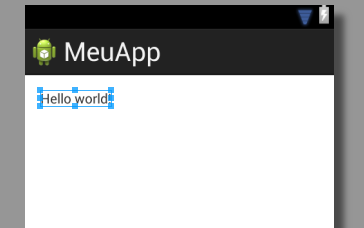
\includegraphics{figuras/3-criando-app.png}
  \caption{Selecionando o Hello world}
  \label{fig:b}
\end{figure}

A tela deverá ficar parecida com a da figura 4.4. Agora arraste um \textit{Text Field -> Plain Text} e um \textit{Form Widgets -> Button} para sua \emph{activity}.

\begin{figure}[H]
  \centering
  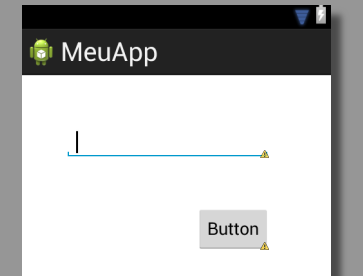
\includegraphics{figuras/4-criando-app.png}
  \caption{\emph{activity} com os elementos colocados na tela}
  \label{fig:a}
\end{figure}

Ao clicar duas vezes no elemento no modo visual, você sera levado ao marcador desse elemento no XML correspondente da \emph{activity}. Clique duas vezes na caixa de texto, o seguinte código será exibido:

\begin{listing}
\inputminted[linenos=true,fontsize=\small,frame=lines, framesep=2mm, tabsize=2,numbersep=5pt]{xml}{src/firstapp/1.xml}
\caption{Código da caixa de texto no arquivo \texttt{activity\_main.xml}}
\end{listing}

Primeiro, na linha 2 modifique o \emph{id} do \emph{Text Field} para um nome mais intuitivo, nesse exemplo chamaremos apenas de \emph{nameField}. O Android definiu que todo novo atributo \emph{id} deve ser precedido de \texttt{@+id/}. O símbolo @ diz para o compilador que estamos acessando os recursos do Android, esses recursos são compilados na classe \texttt{R} automaticamente. O símbolo + diz para o compilador que estamos criando um novo recurso. Por fim, \emph{id} diz que estamos especificando um novo identificador para esse recurso e só então damos o nome a esse identificador.

\begin{framed}
\textbf{Dica:} Existem vários tipos de recursos, porém é importante salientar os diferentes tipos de \emph{id}. Quando referimos aos recursos podemos usar \texttt{@android:id/} para acessar recursos que já estão definidos no sistema Android. Usamos \texttt{@id/} para acessar recursos que já foram definidos no seu projeto. Para criar um novo recurso, usamos \texttt{@+id/}.
\end{framed}

Os outros atributos são para definir o tamanho, alinhamento e margem da caixa de texto. O valor \texttt{wrap\_content} dos atributos \texttt{layout\_width} e \texttt{layout\_height} (largura e altura, linhas 3 e 4) força a \emph{view} a mudar de tamanho automaticamente para abrigar seu conteúdo. Os atributos \texttt{layout\_alignParentLeft} e \texttt{layout\_alignParentTop} servem (linhas 5 e 6) para alinhar essa \emph{view} com a \emph{view} pai dela, dessa forma ficará alinhado com a borda esquerda e com a borda superior do pai. Os atributos \texttt{layout\_marginLeft} e \texttt{layout\_marginTop} (linhas 7 e 8) deslocam o elemento colocando uma margem entre a borda e a \emph{view}, esses valores estarão diferentes pois são computados automaticamente quando a \emph{view} é colocada através do construtor de interfaces. Note que isso só acontecerá caso esteja usando \texttt{RelativeLayout}\footnote{Mais informações na seção 5.3} que é o nosso caso. Por útlimo o atributo \texttt{ems} (linha 9) configura o tamanho da fonte através da unidade de medida Em.

Depois adicione uma \textit{hint} para essa caixa de texto, uma \textit{hint} é algo que vai estar escrito na caixa de texto quando ela estiver vazia, indicando que tipo de texto você pretende que seja escrito nessa caixa de texto, Neste exemplo (linha 10) a \textit{hint} é uma referência a \emph{string} chamada \emph{name} que iremos definir depois.

Depois modifique o código do botão que está no mesmo arquivo, troque o \emph{id} do botão (linha 2), também edite o atributo \texttt{text} (linha 8) para fazer uma referência a uma \emph{string} definida no arquivo de \emph{strings} que iremos chamar de \emph{send\_button}. Por último adicione um atributo \texttt{onClick} (linha 9) que define o método que será chamado quando esse botão for pressionado.

\begin{listing}[H]
\inputminted[linenos=true,fontsize=\small,frame=lines, framesep=2mm, tabsize=2,numbersep=5pt]{xml}{src/firstapp/2.xml}
\caption{Código do botão}
\end{listing}

Agora iremos definir as \emph{strings} usadas anteriormente no arquivo \texttt{res/values/strings.xml}. Abra ele e o modifique para que fique como mostrado no Algoritmo \ref{code:arquivo-strings}.

\begin{listing}
\inputminted[linenos=true,fontsize=\small,frame=lines, framesep=2mm, tabsize=2,numbersep=5pt]{xml}{src/firstapp/3.xml}
\caption{Arquivo de strings com as duas strings adicionadas}
\label{code:arquivo-strings}
\end{listing}

Após terminar abra a classe \texttt{MainActivity.java} localizada na pasta \texttt{src/com.example.meuapp/} do seu projeto e adicione um novo método que chamei de \emph{sendMessage}, ele será responsável por obter o conteúdo da caixa de texto e enviar para uma nova \emph{activity} que irá mostrar esse conteúdo.

\begin{listing}
\inputminted[linenos=true,fontsize=\small,frame=lines, framesep=2mm, tabsize=2,numbersep=5pt]{java}{src/firstapp/4.java}
\caption{Adicionando método à classe MainActivity}
\end{listing}

\begin{framed}
\textbf{Dica:} Isso vai requer você importe a classe View, você pode apertar \texttt{Ctrl+Shit+O} no Eclipse para importar classes que estejam faltando
\end{framed}

\begin{listing}
\inputminted[linenos=true,fontsize=\small,frame=lines, framesep=2mm, tabsize=2,numbersep=5pt]{java}{src/firstapp/4-2.java}
\caption{Exemplo de import de uma classe Android}
\end{listing}

Primeiro, crie um novo \texttt{Intent}\footnote{Documentação Intent: \href{http://developer.android.com/reference/android/content/Intent.html}{http://developer.android.com/reference/android/content/Intent.html}}, um \texttt{Intent} é um objeto que provê uma facilidade para realizar uma ligação entre códigos de diferentes aplicações. O uso mais significante é a inicialização de novas \emph{activities}.

\begin{listing}[H]
\inputminted[linenos=true,fontsize=\small,frame=lines, framesep=2mm, tabsize=2,numbersep=5pt]{java}{src/firstapp/5.java}
\caption{Adicionando uma \texttt{Intent}}
\label{code:obtendo-intent}
\end{listing}

Agora iremos obter o texto que está escrito na caixa para fazer algo com ele, no caso iremos enviar para outra \emph{activity} que irá mostrar esse texto. Como é feito no algoritmo \ref{code:obtendo-intent}.

\begin{listing}[H]
\inputminted[linenos=true,fontsize=\small,frame=lines, framesep=2mm, tabsize=2,numbersep=5pt]{java}{src/firstapp/6.java}
\caption{Obtendo o conteúdo da caixa de texto e enviando para outra \emph{activity}}
\end{listing}

O código na linha 3 está obtendo a referência a caixa de texto usando o método \texttt{findViewById()} passando o \textit{id} da caixa de texto como parâmetro, esse \emph{id} é obtido acessando uma variável estática da classe \texttt{R}  (observe que esse e o mesmo \emph{id} que voce colocou no arquivo xml do layout da \emph{activity}).
Em seguida usando o método \texttt{getText()} da caixa de texto, obtem-se a \emph{string} que foi escrita pelo usuário.

Por fim, essa \emph{string} é colocada no \texttt{Intent} com o método \texttt{putExtra()}, uma \texttt{Intent} pode carregar consigo uma coleção de vários tipos de dados como pares chave-valor chamados \textit{extras}, esse método toma a chave como primeiro parâmetro e o valor no segundo parâmetro.
Para que a próxima \emph{activity} consiga coletar esse valor, você deve definir uma chave para seu \textit{extra} usando uma constante pública. Para isso adicione a definição de \texttt{EXTRA\_MESSAGE} no topo da sua classe \texttt{MainActivity}.

\begin{listing}[H]
\inputminted[linenos=true,fontsize=\small,frame=lines, framesep=2mm, tabsize=2,numbersep=5pt]{java}{src/firstapp/7.java}
\caption{Constante como chave para um extra}
\end{listing}

Agora você deve criar uma nova \emph{activity}, para isso vá em \textit{File -> New -> Other -> Android Activity} e selecione \textit{Blank Activity}. Preencha a próxima janela como na figura 4.8, depois clique \textit{Finish}. 

\begin{figure}[H]
  \centering
  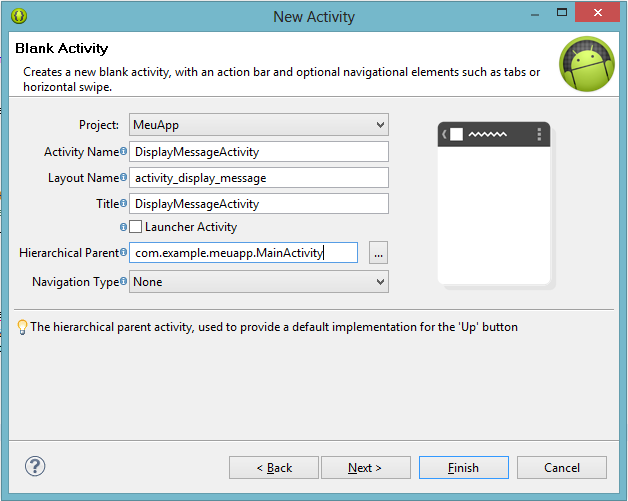
\includegraphics[width=1\textwidth]{figuras/5-criando-app.png}
  \caption{Criando uma nova \emph{activity}}
  \label{fig:e}
\end{figure}

Observe a figura 4.8. Em \emph{Project} você vai especificar o projeto em que a nova \emph{activity} será adicionado. Em \emph{Activity Name} especifique o nome da sua nova \emph{activity}. Em \emph{Layout Name} defina o nome do arquivo XML que contém o \emph{layout} da nova \emph{activity}. A opção \emph{Title} define o título da \emph{activity}, isso pode ser modificado posteriormente no arquivo de \emph{strings} pois o título será definido ali após a criação da \emph{activity}. A opção \emph{Launcher Activity} ficará desmarcada pois essa \emph{activity} não será usada para inicializar o aplicativo. Em \emph{Hierarchical Parent} você vai definir o pai da nova \emph{activity}, isso é usado para o Android implementar corretamente para qual \emph{activity} o botão de voltar irá voltar. Por último \emph{Navigation Type} deixe como \emph{None} pois só queremos o \emph{design} padrão. Clique em \emph{Finish} para criar a nova \emph{activity}.
 
 % nota/dica necessaria?
\begin{framed}
\textbf{Dica:} O Eclipse adiciona automaticamente \emph{activities} criadas por esse método no \emph{Manifest}. Observe no \emph{Manifest} como é feito caso você precise adicionar manualmente.
\end{framed}


Abra a nova classe que foi criada junto com a \emph{activity}. A classe já vem com alguns métodos implementados, alguns não serão necessários para esse aplicativo e serão explicados em outras seções, mas mantenha-os na classe. Todas as classes que são subclasses de \emph{Activity} precisam implementar o método \texttt{onCreate()}\footnote{\href{http://developer.android.com/reference/android/app/Activity.html\#onCreate(android.os.Bundle)}{http://developer.android.com/reference/android/app/Activity.html\#onCreate(android.os.Bundle)}} que define o procedimento a ser executado quando a \emph{activity} é criada.

Agora, precisamos extrair os dados enviados a essa \emph{activity} através do \emph{intent}, você pode obter a referência do \emph{intent} que começou a \emph{activity} chamando o método \texttt{getIntent()}\footnote{\href{http://developer.android.com/reference/android/app/Activity.html\#getIntent()}{http://developer.android.com/reference/android/app/Activity.html\#getIntent()}}.

\begin{listing}[H]
\inputminted[linenos=true,fontsize=\small,frame=lines, framesep=2mm, tabsize=2,numbersep=5pt]{java}{src/firstapp/8.java}
\caption{Obtendo a \emph{string} passada como extra passados através do \texttt{Intent}}
\label{code:obtendo-string-intent}
\end{listing}

Após obter a referência do \emph{intent} que inicou a \emph{activity}, queremos coletar os extras que foram passado junto com ele. Criamos uma \emph{string} que irá armazenar a mensagem que veio junto do \emph{intent} e chamamos o método \texttt{getStringExtra()} passando como parâmetro a chave desse extra, que definimos na classe \texttt{MainActivity}. 
Agora para mostrar a mensagem na tela, você precisa criar um \texttt{TextView}\footnote{\href{http://developer.android.com/reference/android/widget/TextView.html}{http://developer.android.com/reference/android/widget/TextView.html}}, essa \emph{view} serve para mostrar texto. 

\begin{listing}[H]
\inputminted[linenos=true,fontsize=\small,frame=lines, framesep=2mm, tabsize=2,numbersep=5pt]{java}{src/firstapp/9.java}
\caption{Método \texttt{onCreate()} recebendo um \emph{Intent} e mostrando a mensagem}
\end{listing}

As linhas 3, 5 e 6 foram colocadas automaticamente na criação da \emph{activity}, a linha 3 faz uma chamada ao método da superclasse, a linha 6 é um método que inicializa a \emph{Action Bar}, que nesse aplicativo é a barra superior com o nome da \emph{activity} e um menu de opções que já vem pré-programado. Deixamos isso como está.

O algoritmo \ref{code:obtendo-string-intent} foi colocado nas linhas 9 e 10 para obter a referência ao \emph{Intent}. Nas linhas 12-15 criamos um novo \texttt{TextView}, configuramos o tamanho da fonte e atribuímos o texto que será mostrado na tela a \emph{view}, respectivamente. 

Agora que o aplicativo está pronto, é necessário testar, caso tenha um smartphone Android você pode conectá-lo no seu computador e rodar diretamente, senão você deverá rodar em um emulador. Lembrando que para ambos os casos é necessária a instalação do SDK primeiro, acesse \emph{Android SDK Manager} e faça o download do SDK desejado.

Para rodar diretamente no smartphone:
\be
\item Conecte seu smartphone no computador através do cabo USB. Se estiver desenvolvendo no Windows será preciso instalar os drivers USB do seu dispositivo. Se precisar de ajuda para instalar os drivers acesse: \href{http://developer.android.com/tools/extras/oem-usb.html}{OEM USB}\footnote{\href{http://developer.android.com/tools/extras/oem-usb.html}{http://developer.android.com/tools/extras/oem-usb.html}}
\item Ative o modo \emph{USB Debugging} no dispositivo
	\bi
	\item Para Android 3.2 ou mais antigos, a opção deve estar em \textit{Configurações -> Aplicativos	 -> Desenvolvimento}
	\item Para Android 4.0 e 4.1, a opção está em \textit{Configurações -> Opções do desenvolvedor}
	\item Para Android 4.2 e mais novos, a opção está escondida por padrão, para mostrar a opção você deve entrar em \textit{Sobre o telefone} e clicar em \textit{Número da versão} 7 vezes, ao retornar para tela anterior deverá aparecer \textit{Opções do desenvolvedor}
	\ei
\ee

\begin{framed}
\textbf{Dica:} Caso ocorra o erro \emph{Launch error: adb rejected command: device not found}. Verifique se o aparelho está conectado e se os drivers estão instalados corretamente. Na área de notificações do aparelho deve ter uma notificação escrita: \emph{Android debugging enabled}. 
\end{framed}


\newpage 
Para rodar no emulador:
\be
\item Abra o \textit{SDK Manager} através do Eclipse em: \textit{Window -> Android SDK Manager}
\item Verifique se, para Android 4.2.2 (API 17) ou outro desejado os seguintes pacotes estejam instalados
	\bi
	\item \textit{SDK Platform} e;
	\item \textit{ARM EABI v7a System Image} ou;
	\item \textit{Intel x86 Atom System Image}
	\ei
\item Verifique também se na aba \textit{Tools}, os pacotes \textit{Android SDK Tools} e \textit{Android SDK Platform-tools} estão instalados
\item Agora é necessário criar um AVD (Android Virtual Device\footnote{\href{http://developer.android.com/tools/devices/index.html}{http://developer.android.com/tools/devices/index.html}}). No Eclipse acesse o menu \textit{Window -> Android Virtual Device Manager} 
\item No AVD Manager clique em \emph{New}
\item Complete as informações do AVD, especificando um aparelho, nome, plataforma, espaço de armazenamento, quantidade de memória RAM. Em \emph{Device} haverá opções pré-configuradas de aparelhos do google, os \emph{Nexus}, e opções genéricas de acordo com tamanho de tela. Em \emph{Target} você deverá escolher a versão do sistema Android que deseja. Em alguns casos você poderá decidir pela CPU caso deseje ARM ou Intel Atom x86. A quantidade de RAM no Windows fica limitada a 768MB, mais que isso pode acarretar em erros no sistema.

\item Clique \emph{Create AVD}
\item Ainda na janela \emph{Android Virtual Device Manager} selecione o novo AVD e clique \emph{Start}
\item Quando o emulador terminar de carregar, destrave a tela do emulador, usando o mouse.
\ee

Agora para rodar o aplicativo basta clicar em \emph{Run} na barra de tarefas do Eclipse e selecionar \textit{Android Application} na janela \emph{Run as}. O Eclipse irá instalar o APK e abrir o aplicativo automaticamente, no dispositivo ou no emulador. As figuras 4.6, 4.7 e 4.8 mostram a execução do aplicativo.

\begin{figure}[H]
  \centering
  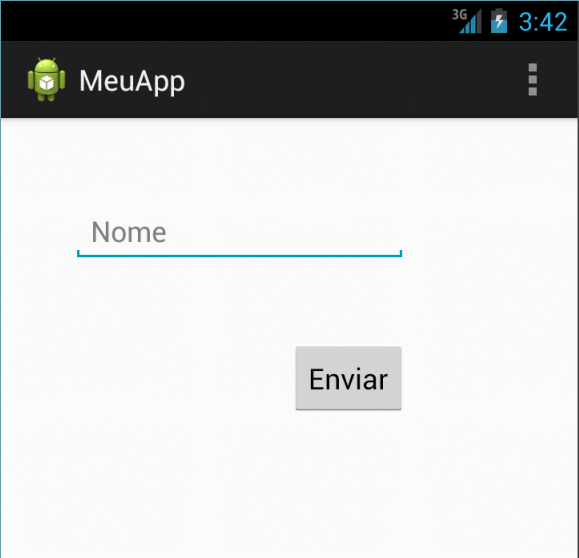
\includegraphics[width=.4\textwidth]{figuras/6-criando-app.png}
  \caption{Primeira tela do primeiro aplicativo}
  \label{fig:f}
  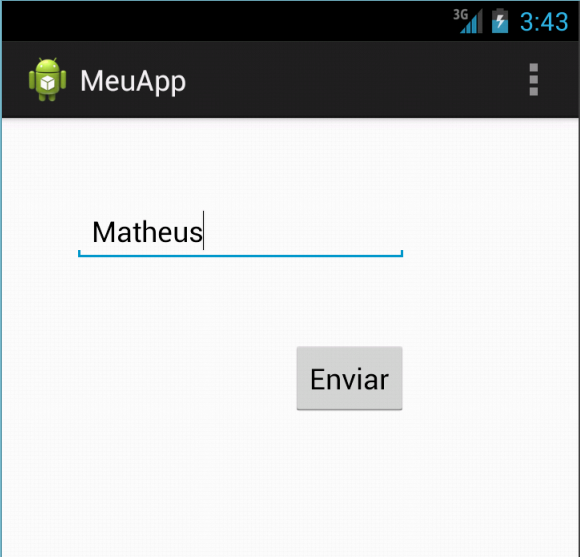
\includegraphics[width=.4\textwidth]{figuras/7-criando-app.png}
  \caption{Primeira tela após escrever texto na caixa de texto}
  \label{fig:g}
\end{figure}
\begin{figure}[H]
  \centering
  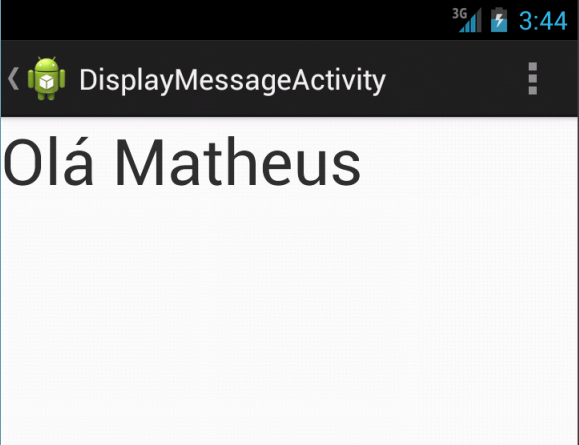
\includegraphics[width=.4\textwidth]{figuras/8-criando-app.png}
  \caption{Segunda tela mostrando a mensagem enviada}
  \label{fig:h}
\end{figure}

%%%%%%% DESIGN %%%%%%%%%%
\cha{design}{Design}

%%% ACTIVITY %%%
\section{Activity}
Enquanto um usuário navega pelas variadas telas de um aplicativo, sai dele e volta depois, as instâncias de uma \emph{activity} transitam dentre diferentes estados em seu ciclo de vida. Quando um aplicativo é iniciado, uma \emph{activity} inicial é criada o sistema invoca métodos específicos que correspondem a criação dessa \emph{activity}. Durante todo o ciclo de vida vários métodos são chamados, e todos eles correspondem a diferentes estágios desse ciclo de vida. 

Observe na imagem abaixo os métodos correspondentes a cada estado da vida de uma \emph{activity}, quando ela é criada o método \texttt{onCreate()} é o responsável pela configuracão inicial. O sistema ao criar uma nova instância de uma \emph{activity}, cada método muda o estado da \emph{activity} um degrau pra cima na pirâmide. 

% COLOCAR FONTE: http://developer.android.com/training/basics/activity-lifecycle/starting.html %
\begin{figure}[H]
  \centering
  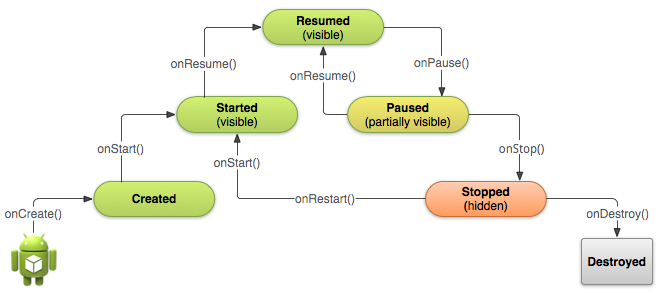
\includegraphics[width=1\textwidth]{figuras/design/basic-lifecycle.png}
  \caption{Ciclo de vida de uma \emph{activity} }
  \label{fig:e}
\end{figure}

Assim que o usuário começa a sair da \emph{activity}, o sistema invoca outros métodos que movem o estado para níveis mais baixos da pirâmide para começar a desmontar a \emph{activity}. Em alguns casos a \emph{activity} irá apenas ir até certo ponto e esperar (por exemplo quando o usuário troca para outro aplicativo) tal que ela possa voltar de onde parou caso o usuário volte. 

 Não são todos métodos que precisam ser implementados pois isso irá depender da complexidade do seu aplicativo. É importante salientar porém que, implementar esses métodos irá garantir que seu aplicativo se comporte de maneira correta, por exemplo você deve garantir que:
 \bi
 \item Seu aplicativo não falhe quando o usuário receber uma chamada telefônica ou quando o usuário troca de aplicativo;
 \item Seu aplicativo não consuma recursos do sistema enquanto não estiver sendo usado;
 \item Seu aplicativo não perca o progresso do usuário; e
 \item Seu aplicativo não falhe ou perca o progresso do usuário quando a tela rotaciona entre retrato e paisagem.
\ei

Apenas três dentre os estados são estáticos, isto é, a \emph{activity} pode ficar nesse estado por um longo período de tempo:


Retomado \emph{(Resumed)}
	
\hspace*{5mm} Nesse estado a \emph{activity} está em primeiro plano e o usuário pode interagir com ela.
	
Pausado \emph{(Paused)}
	
\hspace*{5mm} Nesse estado a \emph{activity} está parcialmente obscurecida por outra \emph{activity} - a outra \emph{activity} que está em primeiro plano é semi-transparente ou não ocupa todo espaço da tela. A \emph{activity} quando pausada não consegur interagir com o usuário e não executa nenhum código.
	
Parado \emph{(Stopped)}
	
\hspace*{5mm} Nesse estado a \emph{activity} está completamente oculto e não está visível para o usuário, está em plano de fundo. Quando está parada, uma instância de uma \emph{activity} e toda informação de seu estado tais como variáveis são mantidos, porém a \emph{activity} não executa nenhum código.
	
\section{Especifique a \emph{activity} que inicia seu aplicativo}

Quando um usuário abre um aplicativo, o sistema chama o método \texttt{onCreate()} da \emph{activity} que foi declarada como sendo a iniciadora do aplicativo. Você pode definir qual \emph{activity} que vai iniciar seu aplicativo no arquivo \texttt{AndroidManifest.xml} que está no diretório raíz do seu projeto.

 A \emph{activity} que inicia seu aplicativo deve ser declarada no manifesto com um \texttt{<intent-filter>}\footnote{Documentação \texttt{<intent-filter>}: \href{http://developer.android.com/guide/topics/manifest/intent-filter-element.html}{http://developer.android.com/guide/topics/manifest/intent-filter-element.html}} que inclui a \texttt{<action>} MAIN e a \texttt{<category>} LAUNCHER. Por exemplo:
 
\begin{listing}[H]
\inputminted[linenos=true,fontsize=\small,frame=lines, framesep=2mm, tabsize=2,numbersep=5pt]{xml}{src/design/launcher-manifest.xml}
\caption{Exemplo de \emph{Launcher activity}}
\end{listing}

%dica
\begin{framed}
\textbf{Dica:} Quando você cria um projeto Android no Eclipse, por padrão é incluida uma classe \emph{activity} que está declarada no manifesto com esse filtro.
\end{framed}

%%% Tipos de Layout %%%
\section{Tipos de \emph{Layout}}
Uma \emph{Activity} contém \emph{Views} e \emph{ViewGroups}. Uma \emph{view} é um elemento que têm presença na tela do dispositivo tais como botões, textos, imagens e etc. Um \emph{ViewGroup} por sua vez é um elemento agrupador de \emph{views} que provê um \emph{layout} na qual você pode ajustar a ordem e aparição das \emph{views}. 

\subsection{LinearLayout}

O \texttt{LinearLayout} arranja \emph{views} em uma única coluna ou uma única linha, desse modo as \emph{views} podem ser arranjadas verticalmente ou horizontalmente. Como mostrado na figura 5.2:

\begin{figure}[H]
  \centering
  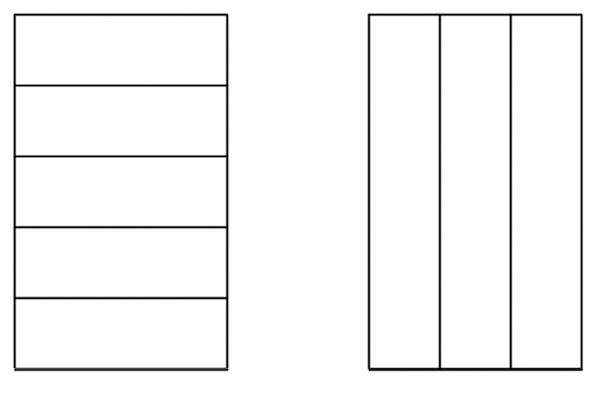
\includegraphics[width=.45\textwidth]{figuras/design/linearlayout.jpg}
  \caption{\texttt{LinearLayout} vertical (à esquerda) e horizontal (à direita)}
  \label{fig:e}
\end{figure}

\emph{ViewGroups} também podem ser agrupados entre si para a criação de layouts mais complexos, por exemplo é possível agrupar um \texttt{LinearLayout} horizontal dentro de um vertical dessa forma é possível colocar \emph{views} lado a lado em uma camadas do \texttt{LinearLayout} vertical, representada na figura 5.3.

\begin{figure}[H]
  \centering
  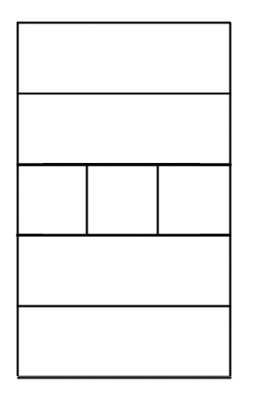
\includegraphics[width=.25\textwidth]{figuras/design/linearlayout-composto.jpg}
  \caption{\texttt{LinearLayout} composto}
  \label{fig:e}
\end{figure}

\subsection{RelativeLayout}

O \texttt{RelativeLayout} permite especificar como as \emph{views} são posicionadas uma em relação a outra. Cada \emph{view} embutida no interior de um \texttt{RelativeLayout} tem atributos que permitem o seu alinhamento com outras \emph{views}. Esses atributos podem ser encontrados na \href{http://developer.android.com/reference/android/widget/RelativeLayout.LayoutParams.html}{documentação}\footnote{ \href{http://developer.android.com/reference/android/widget/RelativeLayout.LayoutParams.html}{http://developer.android.com/reference/android/widget/RelativeLayout.LayoutParams.html}}

\begin{figure}[H]
  \centering
  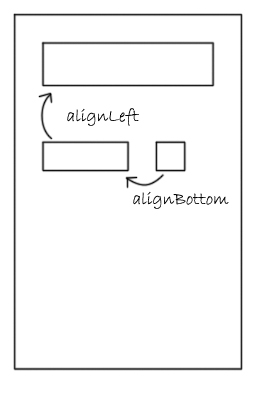
\includegraphics[width=.25\textwidth]{figuras/design/relativelayout.jpg}
  \caption{Exemplo de \texttt{RelativeLayout}}
  \label{fig:e}
\end{figure}

Novamente cabe comentar que é possível aninhar diferentes \emph{ViewGroups} para formar um \emph{layout} com maior complexidade.

\subsection{FrameLayout}

O \texttt{FrameLayout} é o mais simples e eficiente tipo de \emph{layout}, pode ser usado apenas para mostrar uma \emph{view} ou \emph{views} que se sobrepõem. Geralmente é usado como um recipiente para os \texttt{Fragments}\footnote{Mais informações na seção XXXXXX}.

Uma \emph{view} definida em um \texttt{FrameLayout} sempre será colocado no canto superior esquerdo da tela do dispositivo ou do \emph{ViewGroup} a que pertence o \texttt{FrameLayout}. Se mais de uma \emph{view} foi definida elas serão empilhadas uma em cima da outra. Isso significa que a primeira \emph{view} adicionada ao \texttt{FrameLayout} será mostrada na base da pilha, e a última adicionada será mostrada no topo.

Você pode fazer com que as \emph{views} não sobreponham as outras usando o atributo \texttt{layout\_gravity}\footnote{\href{http://developer.android.com/reference/android/widget/FrameLayout.LayoutParams.html}{http://developer.android.com/reference/android/widget/FrameLayout.LayoutParams.html}}, dessa forma uma \emph{view} pode ficar posicionada na borda inferior e outra na borda superior e não ficarem sobrepostas.

É possível posicionar as \emph{views} dentro de um \texttt{FrameLayout} usando parâmetros diferentes no \texttt{layout\_gravity}, no exemplo da figura 5.5 existe um \texttt{FrameLayout} com 3 elementos e cada um com parâmetros diferentes. É possivel combinar os parâmetros utilizando a barra reta '|'.

\begin{figure}[H]
  \centering
  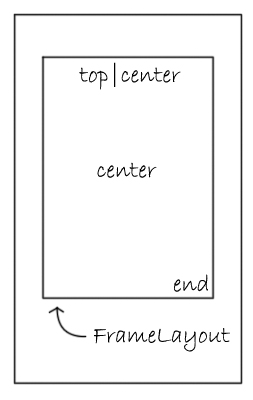
\includegraphics[width=.25\textwidth]{figuras/design/framelayout_gravity.jpg}
  \caption{\texttt{FrameLayout} com exemplo de posicionamento usando \texttt{layout\_gravity}}
  \label{fig:e}
\end{figure}

\subsection{TableLayout}

\texttt{TableLayouts} podem ser usadas para apresentar dados tabulados ou alinhar conteúdo como tabelas HTML em uma página web. Um \texttt{TableLayout} é composto de \texttt{TableRows}, uma cada para linha da tabela. Os conteúdos das \texttt{TableRows} são as \emph{views} que vão em cada célula da tabela. Cada linha terá zero ou mais células e cada célula pode conter uma \emph{view}. 

O aspecto da \texttt{TableLayout} vai depender de alguns fatores. Primeiro, o número de colunas da tabela inteira vai depender do número de colunas da linha que contém mais colunas. Segundo, a largura de cada coluna é definida como a largura do conteúdo mais largo da coluna. Você pode combinar colunas para formar uma célula maior, mas não pode combinar linhas. Leia mais na \href{http://developer.android.com/reference/android/widget/TableLayout.html}{documentação}\footnote{\href{http://developer.android.com/reference/android/widget/TableLayout.html}{http://developer.android.com/reference/android/widget/TableLayout.html}}

Embora \texttt{TableLayouts} possam ser usados para projetar interfaces, geralmente não é a melhor opção já que são derivadas de \texttt{LinearLayouts}. Se você tem dados que já estão em formato de tabela, como planilhas, então pode ser uma boa opção.

\begin{figure}[H]
  \centering
  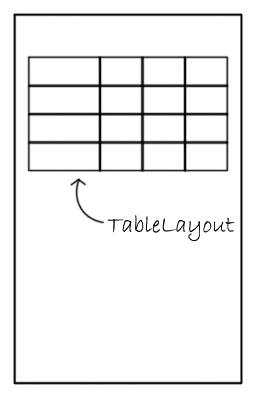
\includegraphics[width=.25\textwidth]{figuras/design/tablelayout.jpg}
  \caption{Exemplo de \texttt{TableLayout}}
  \label{fig:e}
\end{figure}

%%% LIST VIEW %%%%
\section{Listas \texttt{(ListView)}}\footnote{Documentação \texttt{ListView}:\href{http://developer.android.com/reference/android/widget/ListView.html}{http://developer.android.com/reference/android/widget/ListView.html}}
Listas são uma das formas mais simples e poderosas de se mostrar informações ao usuário de forma objetiva. A \texttt{ListView} é capaz de aprensentar uma lista rolável de itens. 

\begin{figure}[H]
  \centering
  
\includegraphics[width=.25\textwidth]{figuras/design/listview-scheme.png}
  \caption{Esquema de uma lista}
  \label{fig:e}
\end{figure}

Um item individual da lista pode ser selecionado, essa seleção pode acionar uma outra tela com detalhes do item.


\begin{figure}[H]
  \centering
  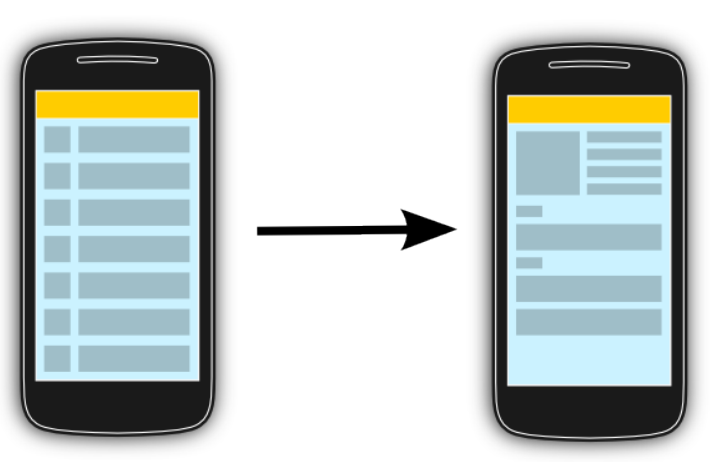
\includegraphics[width=.45\textwidth]{figuras/design/listview-scheme2.png}
  \caption{Detalhes de um elemento da lista}
  \label{fig:e}
\end{figure}

\subsection{Adaptadores}
	Adaptadores são usados para providenciar dados a \emph{views}. O adaptador também define como item da \emph{view} será mostrada. Para \texttt{ListViews} o adaptador define como cada linha será mostrada.
	
	Um adaptador deve extender a classe base \texttt{BaseAdapter}. O Android já tem alguns adaptadores padrão, os mais importantes são o \texttt{ArrayAdapter} e o \texttt{CursorAdapter}. 
	
	O \texttt{ArrayAdapter} é usado para manipular dados em \emph{arrays} ou listas (\texttt{java.util.List}). Já o \texttt{SimpleCursorAdapter} consegue manipular dados em banco de dados.

\subsection{Construção}

A construção desse tipo de design é simples. No arquivo de \emph{layout} da \emph{activity} use o \texttt{LinearLayout} para conter a \texttt{ListView}.

\begin{listing}[H]
\inputminted[linenos=true,fontsize=\small,frame=lines, framesep=2mm, tabsize=2,numbersep=5pt]{xml}{src/design/layout_linear.xml}
\caption{\texttt{LinearLayout} no arquivo de \emph{layout}}
\label{code:linearlayout}
\end{listing}

Se estiver usando o construtor de interface gráfica, pode arrastar uma \texttt{ListView} para dentro do \emph{layout}. Caso contrário pode construir manualmente no arquivo XML do \emph{layout} da \emph{activity}. 

Você deve colocar o \texttt{LinearLayout} como raíz do arquivo XML, o elemento raíz sempre deve conter o atributo \texttt{xmlns:android} como mostrado na linha 2 do algoritmo \ref{code:linearlayout}, não entraremos em detalhes sobre os outros atributos. 

Adicione uma \texttt{ListView}, escreva o código abaixo dentro do \texttt{LinearLayout}. 
\begin{listing}[H]
\inputminted[linenos=true,fontsize=\small,frame=lines, framesep=2mm, tabsize=2,numbersep=5pt]{xml}{src/design/listview.xml}
\caption{Código de uma \texttt{ListView}}
\end{listing}

Você precisa popular a lista, para isso você pode criar um \texttt{string-array} no arquivo \texttt{strings.xml} com os elementos que deseja colocar na lista. Nesse exemplo do algoritmo \ref{code:string-array} foi criado uma lista com nome \texttt{listString} e 4 itens que serão mostrados em forma de lista pela \texttt{ListView}.

\begin{listing}[H]
\inputminted[linenos=true,fontsize=\small,frame=lines, framesep=2mm, tabsize=2,numbersep=5pt]{xml}{src/design/string-array.xml}
\caption{\texttt{string-array} populada com elementos}
\label{code:string-array}
\end{listing}

Finalmente, você deve escrever o código que irá preencher a lista com as \emph{strings}. Como é feito no algoritmo \ref{code:activity-lista} abaixo.

\begin{listing}[H]
\inputminted[linenos=true,fontsize=\small,frame=lines, framesep=2mm, tabsize=2,numbersep=5pt]{java}{src/design/listactivity.java}
\caption{Código de uma \emph{activity} com lista clicável}
\label{code:activity-lista}
\end{listing}

Primeiro, na linha 2, foi criada uma variável do tipo \texttt{ListView} para guardar um ponteiro para a \emph{view} já definida no \emph{layout}.

No método \texttt{onCreate()} você precisa criar e inicializar a lista na sua \emph{activity}. Na linha 10 obtemos as \emph{strings} do \texttt{string-array} e o guardamos na variável \texttt{listStr}. Usamos o método \texttt{getResources()} para poder adquirir o ponteiro para os recursos do aplicativo. Na linha 13 conseguimos o ponteiro pra lista e o guardamos na variável criada.

Usamos o adaptador ao chamar o método \texttt{ListView.setAdapter()} nas linhas 16-17  e passamos como parâmetro a criação de um novo adaptador do tipo \texttt{ArrayAdapter}. Para o construtor\footnote{\href{http://developer.android.com/reference/android/widget/ArrayAdapter.html}{http://developer.android.com/reference/android/widget/ArrayAdapter.html}} desse adaptador está sendo passado o contexto atual da \emph{activity}, um \emph{layout} pré-definido do sistema, o \texttt{simple\_list\_item\_1}, e os dados na forma de \emph{array}.

Na linha 22 usamos o método \texttt{ListView.setOnItemClickListener} para configurar uma ação a ser executada quando um item da lista for clicado. Neste exemplo é criado um \texttt{Toast}, o \texttt{Toast} mostra uma mensagem em uma caixa de texto na parte inferior da tela por um curto período de tempo, nesse caso irá mostrar o mesmo texto do item da lista que foi clicado. Uma das aplicações mais comuns é fazer com que ao se clicar em um item da lista, uma nova \emph{activity} seja aberta com detalhes do item.

\begin{figure}[H]
  \centering
  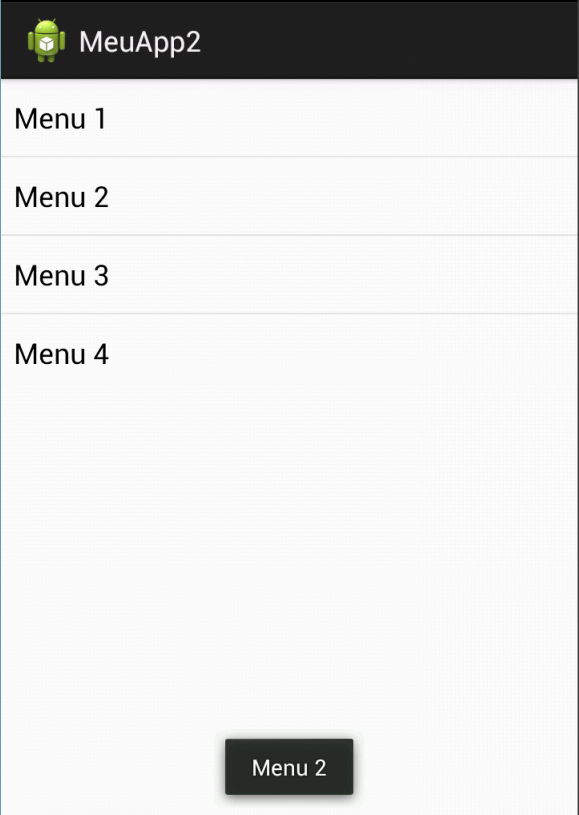
\includegraphics[width=.7\textwidth]{figuras/design/lista.png}
  \caption{Lista simples}
  \label{fig:e}
\end{figure}

A figura 5.9 mostra como ficou o exemplo ao ser executado em um \emph{smartphone}, o item ''Menu 2'' foi clicado e um \texttt{Toast} foi mostrado no momento do clique.

%%% LIST ADAPTER %%%
\section{Listas Compostas}
É possível compor um item da lista colocando mais elementos além de um texto. Para isso você precisa criar um novo arquivo XML que irá definir a customização de cada linha da \texttt{ListView}, nesse exemplo iremos definir um arquivo chamado \texttt{item.xml}, mostrado abaixo.


\begin{listing}[H]
\inputminted[linenos=true,fontsize=\small,frame=lines, framesep=2mm, tabsize=2,numbersep=5pt]{xml}{src/design/item.xml}
\caption{Código do arquivo \texttt{item.xml}}
\label{code:itemxml}
\end{listing}	

O algoritmo \ref{code:itemxml} mostra como você pode fazer a customização de um item da lista. Nesse exemplo há uma pequena imagem à esquerda e dois textos de cores e tamanhos diferentes. 
Para isso primeiro criamos um \texttt{LinearLayout} que irá conter uma \texttt{ImageView} para mostrar a imagem e outro \texttt{LinearLayout} para colocar os dois textos. As cores do textos são configuradas com o atributo \texttt{textColor} e usa o padrão HTML de cores.

Agora você precisa usar um adaptador para mostrar esse layout customizado em cada linha da lista, usaremos a classe \texttt{SimpleAdapter}\footnote{\href{http://developer.android.com/reference/android/widget/SimpleAdapter.html}{http://developer.android.com/reference/android/widget/SimpleAdapter.html}}. Essa classe faz a adaptação de um \texttt{ArrayList} de \texttt{Maps} para um \emph{layout} definido. 

\begin{listing}[H]
\inputminted[linenos=true,fontsize=\small,frame=lines, framesep=2mm, tabsize=2,numbersep=5pt]{java}{src/design/customlist.java}
\caption{Código da lista customizada}
\label{code:custom-list}
\end{listing}	

Observando o algoritmo \ref{code:custom-list}. Na linha 13 criamos um \texttt{ArrayList} de \texttt{Maps}. Na linha 14 e 19 criamos um \texttt{HashMap} onde a chave é uma \emph{string} que identifica o conteúdo, essas chaves serão \emph{userIcon}, \emph{userName} e \emph{userText} respectivamente. Em \emph{userIcon} colocamos uma imagem, essa imagem deve ser colocada nas subpastas da pasta \texttt{drawable} e é acessada através da classe \texttt{R}. Em \emph{userName} colocamos um nome de usuário, por exemplo. Em \emph{userText} poderia ser colocada uma descrição, ou uma frase customizada do usuário mas nesse exemplo foi colocado uma sentença qualquer. Nas linhas 18 e 23 adicionamos o \texttt{Map} criado no \texttt{ArrayList}.

Criamos o \texttt{SimpleAdapter} nas linhas 26-29. Para o construtor passamos o \texttt{ArrayList} de \texttt{Maps} que contém os dados, passamos também o \emph{layout} que definimos anteriormente \texttt{R.layout.item}. Passamos um \emph{array} de \emph{strings} que contém as chaves que serão usadas para obter os dados e por último um \emph{array} de inteiros que contém os \emph{ids} das \emph{views} em que os conteúdos dos \texttt{Maps} serão colocados.

\begin{figure}[H]
  \centering
  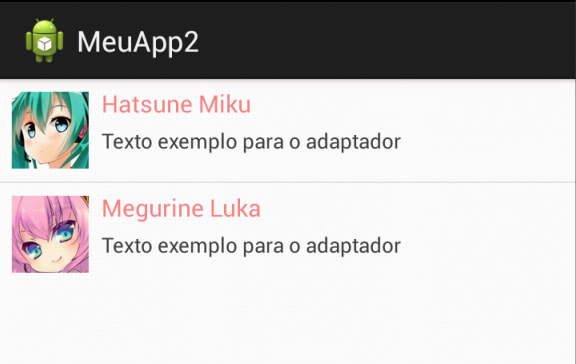
\includegraphics[width=.475\textwidth]{figuras/design/lista-composta.png}
  \caption{Lista Composta}
  \label{fig:e}
\end{figure}

A figura 5.10 mostra como ficou o exemplo acima ao ser executado em um \emph{smartphone}. 

%%% EXPANDABLE LIST %%%
\section{Listas expansíveis \texttt{(ExpandableListView)}}

Listas expansíveis são úteis para agrupar conjuntos de itens semelhantes, funcionam da mesma maneira que as listas comuns e podem ser customizadas.
Comece colocando sua lista no \emph{layout} da \emph{activity} desejada.
	
\begin{listing}[H]
\inputminted[linenos=true,fontsize=\small,frame=lines, framesep=2mm, tabsize=2,numbersep=5pt]{xml}{src/design/exlist.xml}
\caption{Código XML de uma Lista expansível}
\end{listing}	

\begin{framed}
\textbf{Dica:} O atributo \texttt{transcriptMode=''alwaysScroll''} vai fazer com que a lista sempre role até o final quando você expande ou contrai um grupo.
O atrbuto \texttt{listSelector} colore o item da lista quando este é clicado.
\end{framed}

Agora crie 2 novos arquivos XML, um chamado \texttt{list\_item\_parent.xml} e o outro chamado \texttt{list\_item\_child.xml} dentro da pasta \texttt{res/layout}.

\begin{listing}[H]
\inputminted[linenos=true,fontsize=\small,frame=lines, framesep=2mm, tabsize=2,numbersep=5pt]{xml}{src/design/list-item-parent.xml}
\caption{Layout \texttt{list\_item\_parent.xml}}
\end{listing}	

Nesses dois \emph{layouts} teremos apenas uma \texttt{TextView} para abrigar um texto.

\begin{listing}[H]
\inputminted[linenos=true,fontsize=\small,frame=lines, framesep=2mm, tabsize=2,numbersep=5pt]{xml}{src/design/list-item-child.xml}
\caption{Layout \texttt{list\_item\_child.xml}}
\end{listing}	

Em seguida precisamos crare uma classe que irá abrigar os dados dos elementos pai, elementos estes que serão expandidos quando clicados. Nesse exemplo criamos uma classe \emph{Parent}, como mostrado no algoritmo \ref{code:parent}

\begin{listing}[H]
\inputminted[linenos=true,fontsize=\small,frame=lines, framesep=2mm, tabsize=2,numbersep=5pt]{java}{src/design/parent.java}
\caption{Classe \texttt{Parent}}
\label{code:parent}
\end{listing}	

Essa classe contém o texto do item, que será guardado na \emph{string} \texttt{mTitle} e um \texttt{ArrayList} que irá comportar os sub-itens desse item. Os métodos \emph{get} e \emph{set} são simples.

Em seguida, crie uma nova classe, \texttt{CustomAdapter} que será o adaptador da lista expansível para os dados, para esse exemplo estaremos adaptando apenas para o uso de texto. Essa classe deve extender a classe \texttt{BaseExpandableListAdapter}.

\newenvironment{code}{\captionsetup{type=listing}}{}

\begin{code}
\inputminted[linenos=true,fontsize=\small,frame=lines, framesep=2mm, tabsize=2,numbersep=5pt]{java}{src/design/customadapter.java}
\caption{Classe \texttt{CustomAdapter}}
\end{code}

% problema com paragrafo
\parskip 1pt 

Primeiro precisamos de um \texttt{LayoutInflater}\footnote{\href{http://developer.android.com/reference/android/view/LayoutInflater.html}{http://developer.android.com/reference/android/view/LayoutInflater.html}} que irá instanciar o \emph{layout} XML nas \emph{views} correspondentes, e um \emph{array} da classe \texttt{Parents} que criamos anteriormente, esses serão os itens principais da lista.

Na linha 7 no construtor da calsse, usamos o método \texttt{LayoutInflater.from()} para obter o \emph{inflater} do contexto da \emph{activity}. 

Ao extender a classe \texttt{BaseExpandableListAdapter} temos que programar alguns métodos. O método \texttt{getChild()} deve adquirir o ponteiro para um subitem de um item na lista. O método \texttt{getChildId()} deve obter o \emph{id} de um subitem, porém nesse exemplo não temos nada configurado então usamos a própria posição desse subitem como \emph{id} e retornamos \texttt{childPosition}. 

O método \texttt{getChildView} na linha 24 vai atribuir o \emph{layout} dos subitens na linha 28. Na linha 32 obtemos o \texttt{TextView} desse subitem e com o método \texttt{TextView.setText()} atribuimos seu respectivo texto. Esse texto está guardado no \emph{array} chamado \texttt{mArrayChildren} da classe \texttt{Parent}, então a fim de obter esse texto devemos obter o \texttt{Parent} correto. Quando você clica em um item da lista, o Android guarda qual item você clicou no parâmetro \texttt{groupPosition}. Em seguida se obtem o texto de cada subitem pelo parâmetro \texttt{childPosition}.

Outro método importante é o \texttt{getGroupView}, funciona da mesma maneira que \texttt{getChildView} mas configurando os \emph{views} dos itens pai em vez dos subitens.

Para finalizar, você deve construir os objetos na classe da \emph{activity}, nesse exemplo para popular a lista eu coloquei no arquivo de \texttt{strings} alguns fabricantes e modelos de carros, você pode obtê-los no repositório do projeto.

\begin{listing}[H]
\inputminted[linenos=true,fontsize=\small,frame=lines, framesep=2mm, tabsize=2,numbersep=5pt]{java}{src/design/exlist-main.java}
\caption{Construindo a lista expandível na \emph{activity}}
\label{code:listaexp-ac}
\end{listing}	

\newpage

O algoritmo \ref{code:listaexp-ac} é a construção da lista expansível na \emph{activity}, na linha 9-10 obtemos a \emph{view} usando \texttt{findViewById()}. A linha 30-31 são um pouco mais complicadas, primeiro é preciso obter o \emph{id} do \texttt{string-array} que é subitem do item atual no laço de repetição. Para isso usamos \texttt{getResources().getIdentifier()} para obter o \emph{id} do subitem a partir do nome do item pai. Em seguida podemos acessar o \texttt{string-array} normalmente como é feito na linha 31.

 Na linha 41 usamos o \texttt{CustomAdapter} que criamos anteriormente.

\begin{figure}[H]
  \centering
  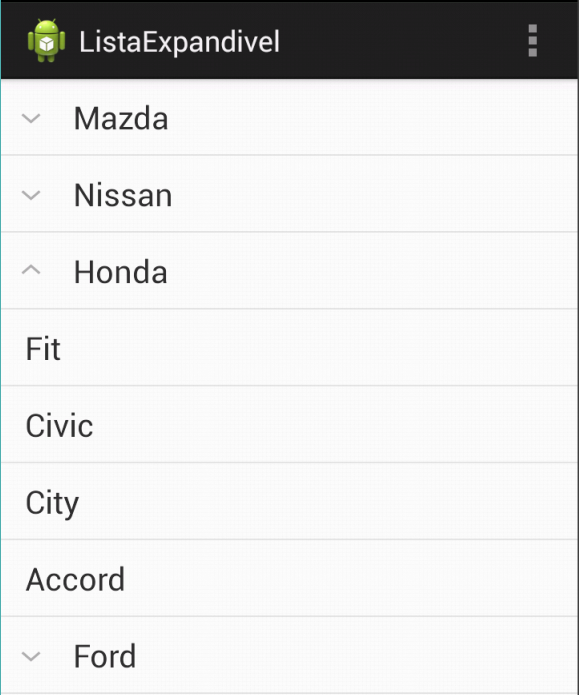
\includegraphics[width=.475\textwidth]{figuras/design/listaexpandivel.png}
  \caption{Exemplo de lista expansível rodando em um \emph{smartphone}}
  \label{fig:e}
\end{figure}

%%% GRADES E IMAGENS %%%
\newpage
\section{Grades \texttt{(GridView)} e imagens \texttt{ImageView}}

Grades são úteis para mostrar imagens e fotos como uma galeria, ou permitir a seleção de categorias semelhante a uma lista. A idéia é ter elementos lado a lado para mostrar ou para selecionar e mostrar mais detalhes. Basicamente funciona como uma grade bi-dimensional que pode ser arrastada para os lados ou de cima pra baixo. 

\begin{figure}[H]
  \centering
  
\includegraphics[width=.475\textwidth]{figuras/design/gridview.png}
  \caption{Esquema de um \texttt{GridView}}
  \label{fig:e}
\end{figure}

Comece colocando um \texttt{GridView}\footnote{\href{http://developer.android.com/reference/android/widget/GridView.html}{http://developer.android.com/reference/android/widget/GridView.html}} no \emph{layout} de sua \emph{activity}.

\begin{listing}[H]
\inputminted[linenos=true,fontsize=\small,frame=lines, framesep=2mm, tabsize=2,numbersep=5pt]{xml}{src/design/gridview.xml}
\caption{Layout do \texttt{GridView}}
\end{listing}	

Vamos criar uma nova classe que será o adaptador de imagens para o \texttt{GridView}, chamemos a classe de \texttt{ImageAdapter}, ela é mostrada no algoritmo \ref{code:image-adapter}.

\begin{listing}[H]
\inputminted[linenos=true,fontsize=\small,frame=lines, framesep=2mm, tabsize=2,numbersep=5pt]{java}{src/design/imageadapter.java}
\caption{Classe \texttt{ImageAdapter}}
\label{code:image-adapter}
\end{listing}	

A classe \texttt{ImageAdapter} deve ser subclasse da classe \texttt{BaseAdapter}\footnote{\href{http://developer.android.com/reference/android/widget/BaseAdaptfer.html}{http://developer.android.com/reference/android/widget/BaseAdapter.html}}. Temos, como variável pública, um \emph{array} das imagens que queremos colocar na grade. Como todo \emph{id} de um recurso da classe \texttt{R} é um inteiro, criamos um \emph{array} de inteiros. Note que estamos considerando que todas as imagens já foram devidamente colocadas na pasta \texttt{drawable}.

O método mais importante é o método \texttt{getView()}. Nele criamos uma nova \texttt{ImageView}\footnote{\href{http://developer.android.com/reference/android/widget/ImageView.html}{http://developer.android.com/reference/android/widget/ImageView.html}} para abrigar a imagem que queremos colocar na grade. Em seguida configuramos alguns parâmetros desse \texttt{ImageView}, o método \texttt{ImageView.setImageResource()} é responsável por estabelecer um \texttt{drawable} como conteúdo do \texttt{ImageView}. Já o método \texttt{View.setLayoutParams()} configura os parâmetros de \emph{layout} associados com essa \emph{view}, note que para esse método passamos parâmetros de \emph{layout} de uma \texttt{GridView}, que por sua vez recebe \texttt{(200,200)} como largura e altura de um elemento da grade.

  \texttt{ImageView.setScaleType} controla como a imagem deve ser redimensionada para condizer com o tamanho do \texttt{ImageView}, \texttt{ImageView.ScaleType}\footnote{\href{http://developer.android.com/reference/android/widget/ImageView.ScaleType.html}{http://developer.android.com/reference/android/widget/ImageView.ScaleType.html}} são as formas disponíveis para escalar a imagem.

Agora basta criar a grade em sua \emph{activity}.

\begin{listing}[H]
\inputminted[linenos=true,fontsize=\small,frame=lines, framesep=2mm, tabsize=2,numbersep=5pt]{java}{src/design/grade-activity.java}
\caption{\emph{activity} com grade}
\end{listing}	

Exemplo acima rodando em um \emph{smartphone} na figura 5.13:

\begin{figure}[H]
  \centering
  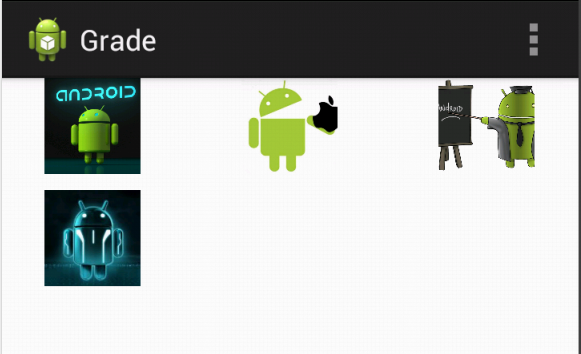
\includegraphics[width=.475\textwidth]{figuras/design/grade-exemplo1.png}
  \caption{Demonstração de um \texttt{Grid view}}
  \label{fig:e}
\end{figure}

Para complementar, você pode fazer com que a imagem abra em tela cheia quando clicada na view, para isso é necessário que você passe o \emph{id} do recurso do \texttt{GridView} para uma nova \emph{activity} que irá mostrar a imagem em tela cheia.
Para isso precisamos criar um novo \emph{layout} XML, a qual chamaremos de \texttt{full\_image.xml}, nele teremos apenas uma \texttt{ImageView} e um \texttt{TextView} que será uma pequena legenda da imagem.

\begin{listing}[H]
\inputminted[linenos=true,fontsize=\small,frame=lines, framesep=2mm, tabsize=2,numbersep=5pt]{xml}{src/design/full-image.xml}
\caption{Layout \texttt{full\_image.xml}}
\end{listing}	

Note que para o \texttt{TextView} usaremos o atributo \texttt{layout\_width} como \texttt{fill\_parent} e \texttt{layout\_height} como \texttt{40dp}, dessa forma criamos um pequeno retângulo de altura fixa mas de forma que a largura preecha a tela completamente. O atributo \texttt{background} com o valor \texttt{\#55555555} faz com que a cor do retângulo seja cinza com transparência, já que o parâmetro \emph{alfa} também tem valor 0x55. Também deixamos o texto com cor branca com o atributo \texttt{textColor}.

Em seguida, crie uma nova classe chamada \texttt{FullImageActivity}, essa é a \emph{activity} que vai mostrar a imagem em tela cheia. A construção da classe é simples, você deve apenas obter o \emph{id} da imagem passado como \emph{extra} através do \texttt{intent} e então obter essa imagem da classe \texttt{ImageAdapter}.

\begin{listing}[H]
\inputminted[linenos=true,fontsize=\small,frame=lines, framesep=2mm, tabsize=2,numbersep=5pt]{java}{src/design/FullImageActivity.java}
\caption{Classe \texttt{FullImageActivity}}
\end{listing}	 	 	

\begin{listing}[H]
\inputminted[linenos=true,fontsize=\small,frame=lines, framesep=2mm, tabsize=2,numbersep=5pt]{java}{src/design/grid-activity-p2.java}
\caption{Código da \emph{activity} após as modificações}
\label{code:act-fullimage}
\end{listing}	 

No algoritmo \ref{code:act-fullimage}, configuramos um \texttt{View.setOnItemClickListener()} de forma que quando uma imagem da grade for clicada, um \texttt{Intent} seja enviado a uma nova \emph{activity} que por sua vez ficará encarregada de mostrar a imagem em tela cheia.  Quando um item é clicado conseguimos obter a posição dele na grade com o parâmetro \texttt{pos} da função \texttt{onItemClick()}, essa posição é equivalente ao \emph{id} da imagem no \emph{array} criado na classe \texttt{ImageAdapter}.  A \texttt{FullImageActivity} por sua vez recebe esse \texttt{Intent} que possui o \emph{id} da imagem que deve ser mostrada e configura o \texttt{ImageView} de acordo. 

\begin{figure}[H]
  \centering
  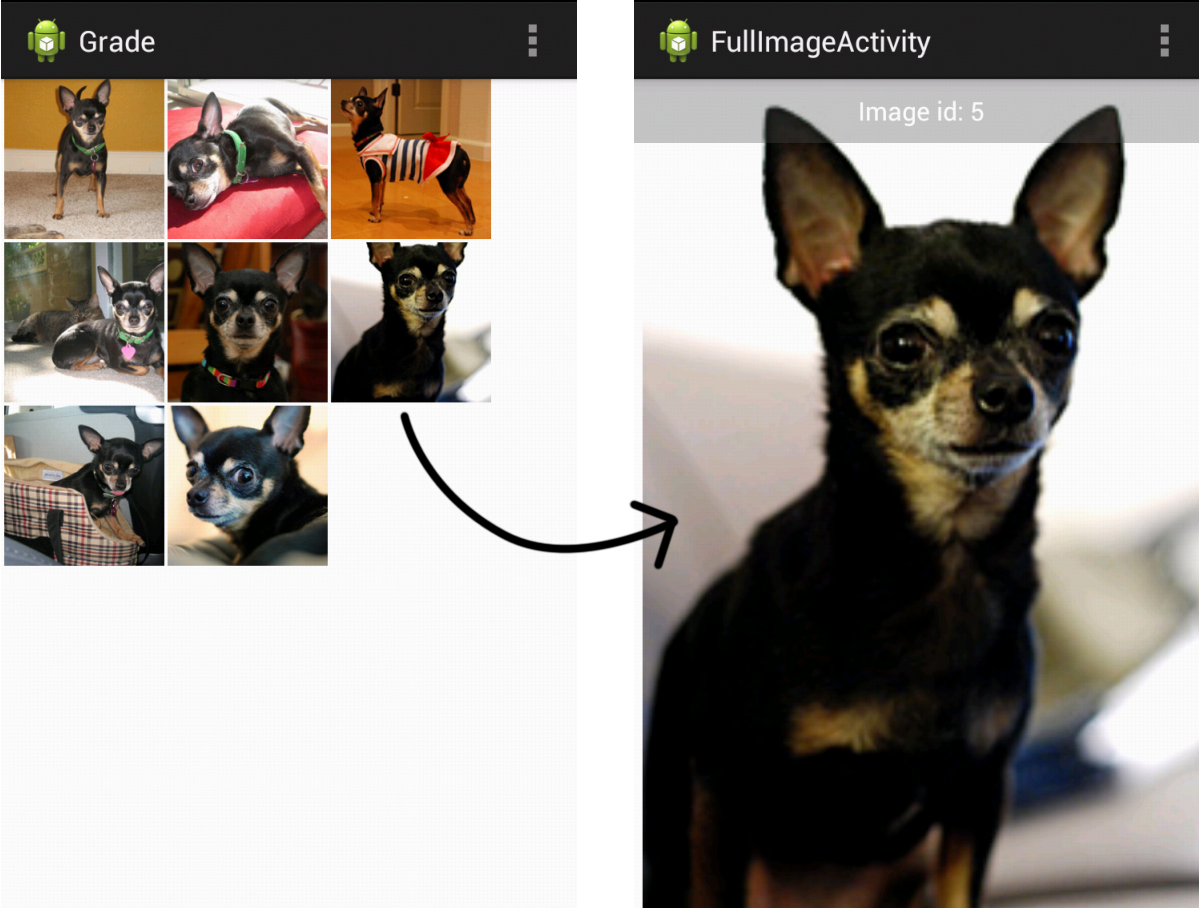
\includegraphics[width=.80\textwidth]{figuras/design/grid-fullimage.jpg}
  \caption{Exemplo \texttt{GridView} com imagem em tela cheia}
  \label{fig:e}
\end{figure}

%% FRAGMENTOS %%
\section{Fragmentos}

Fragmentos são a solução do Android para criar interfaces de usuário modulares, eles vivem dentro das \emph{activity} e uma \emph{activity} pode conter vários fragmentos. Assim como as \emph{activity} os fragmentos possuem um ciclo de vida. %% EXPLICAR MELHOR %%.

Dentre as vantagens de um fragmento estão:
\bi
	\item Modularidade e reuso de código
	\item Habilidade de construir interfaces com múltiplos painéis
	\item Facilidade de construir aplicativos para celulares e tablets
\ei

O primeiro conceito a ser coberto é como construir um fragmento, comece definindo o \emph{layout} do fragmento.

Um layout bem simples, apenas com um botão para efeito de demonstração. Agora crie uma classe \texttt{BasicFragment}

\begin{listing}[H]
\inputminted[linenos=true,fontsize=\small,frame=lines, framesep=2mm, tabsize=2,numbersep=5pt]{java}{src/design/basicfragment.java}
\caption{Classe \texttt{BasicFragment}}
\end{listing}	

Caso você esteja desenvolvendo para API menores que 11 (HoneyComb 3.0) você vai precisar usar a API de retrocompatibilidade que o Google providenciou para essas APIs, você precisa importar a classe de suporte: \mint{java}|import android.support.v4.app.Fragment;|

%% diferença chave? %%
% One of the key differences between a Fragment and an Activity is that Fragments instantiate their Views inside the onCreateView() callback and Activities instantiate their Views using the setContentView() method inside of the onCreate() callback. Fragments also have to manually instantiate their Views using an instance of LayoutInflater, which is provided to the onCreateView() method for convenience. %%

%% Another difference is that a Fragment is not a subclass of Context. This means that a Fragment can not be launched as a component inside your app and therefore always has to live inside of an Activity. This also means that whenever you need a Context inside of a Fragment, you need to get access to the parent Activity. You can do this by using the getActivity() method as we have done in the Fragment button's OnClickListener callback. You need to watch out because getActivity() can return null depending on where the Fragment is in the Activity's lifecycle. So, you should also include a check to see if the Activity is null before you use it. %%

Agora para incluir o fragmento na \emph{activity} existem duas opções. A primeira é inlcuir o fragmento no XML da \emph{activity} como você faria com qualquer \texttt{view}.

\begin{listing}[H]
\inputminted[linenos=true,fontsize=\small,frame=lines, framesep=2mm, tabsize=2,numbersep=5pt]{xml}{src/design/fragment-activity.xml}
\caption{Layout da \emph{activity} com um fragmento}
\end{listing}	

Você pode usar o \texttt{<fragment>} quantas vezes quiser para incluir múltiplos fragmentos.
Note que você precisa usar um nome qualificado em \texttt{android:name}, veja mais na documentação oficial: \href{http://developer.android.com/guide/topics/manifest/activity-element.html\#nm}{activity-element}\footnote{\href{http://developer.android.com/guide/topics/manifest/activity-element.html\#nm}{http://developer.android.com/guide/topics/manifest/activity-element.html\#nm}}

Novamente, caso esteja desenvolvendo para APIs menores que 11, você vai precisar fazer a \emph{activity} extender a classe \texttt{FragmentActivity} e importar a classe de suporte: \mint{java}|import android.support.v4.app.FragmentActivity;|
\mint{java}|public class MainActivity extends FragmentActivity|


Simplesmente configurando a \emph{activity} para usar o fragmento vai fazer com que o fragmento seja adicionado e renderizado na tela, entretanto você deve querer ter mais controle de quando e como seus fragmentos serão adicionados durante o curso do seu aplicativo. Para isso existe uma maneira alternativa de adicionar o fragmento em tempo de execução. A fim de adicionar o fragmento em tempo de execução você precisa fazer uma mudança no layout da \emph{activity}:

\begin{listing}[H]
\inputminted[linenos=true,fontsize=\small,frame=lines, framesep=2mm, tabsize=2,numbersep=5pt]{xml}{src/design/framelayout.xml}
\caption{Layout da \emph{activity} com o \texttt{FrameLayout}}
\end{listing}	

E uma mudança na \emph{activity} que vai mostrar o fragmento:

\begin{listing}[H]
\inputminted[linenos=true,fontsize=\small,frame=lines, framesep=2mm, tabsize=2,numbersep=5pt]{java}{src/design/activity-frag-dyn.java}
\caption{\emph{activity} com adição dinâmica de fragmento}
\end{listing}	

E dessa forma obtemos o mesmo resultado, porém com a adição dinâmica do fragmento, você pode experimentar e fazer com que o botão remova um fragmento e coloca outro diferente no lugar.

%% TABS %%

\section{Abas (\emph{Tabs})}
	Existem diversas maneiras de criar uma interface com abas no Android, uma delas é usando as interfaces \texttt{TabHost} e \texttt{TabWidget}, outra é imitando o comportamento usando apenas \texttt{Fragments}. 

	%% TABHOST TABWIDGET %%	
	\subsection{Usando \texttt{TabHost} e \texttt{TabWidget}}
	
	Abas usando essas interfaces são suportados por todas as versões do android	
	Vamos criar uma interface com abas seguindo esse esquema:
	
	\begin{figure}[H]
	  \centering
	  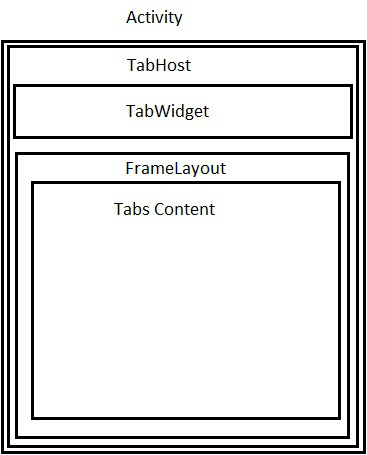
\includegraphics[width=.275\textwidth]{figuras/design/tabs1.jpg}
	  \caption{Esquema da interface com abas}
	  \label{fig:e}
	\end{figure}
	
	Primeiro precisamos criar uma \emph{activity} que servirá como recipiente para as abas e seu conteúdo. O \texttt{TabWidget}\footnote{\href{http://developer.android.com/reference/android/widget/TabWidget.html}{http://developer.android.com/reference/android/widget/TabWidget.html}} é o controle de seleção das abas. Todo conteúdo das abas ficará contido dentro do \texttt{FrameLayout}, é nele que as respectivas \emph{activities} serão mostradas. O \texttt{TabHost}\footnote{\href{http://developer.android.com/reference/android/widget/TabHost.html}{http://developer.android.com/reference/android/widget/TabHost.html}} por sua vez serve como um recipiente para o \texttt{TabWidget} e o \texttt{FrameLayout}.
	
	Crie uma nova \emph{activity}, a chamaremos de \texttt{TabLayoutActivity}. No XML que define o \emph{layout} da \emph{activity}, insira o \texttt{TabHost}, o \texttt{TabWidget} e \texttt{FrameLayout} como mostrado no algoritmo abaixo.
	
	\begin{listing}[H]
	\inputminted[linenos=true,fontsize=\small,frame=lines, framesep=2mm, tabsize=2,numbersep=5pt]{xml}{src/design/activity-tab-host.xml}
	\caption{\emph{Layout} da \emph{activity} \texttt{TabHostLayout}}
	\label{code:layout-tabhost}
	\end{listing}
	
	Agora precisamos definir o \emph{layout} dos fragmentos, isto é, o \emph{layout} de cada aba. Para simplificar o exemplo, as abas só terão um fundo colorido, de cores diferentes. Para isso usa-se o atributo \texttt{background}.
	
	\begin{listing}[H]
	\inputminted[linenos=true,fontsize=\small,frame=lines, framesep=2mm, tabsize=2,numbersep=5pt]{xml}{src/design/tab-fragment.xml}
	\caption{\emph{Layout} do fragmento da aba.}
	\end{listing}
	
	Precisamos definir as classes de cada fragmento de aba. Cada classe deverá extender a classe \texttt{Fragment} e inflar seu \emph{layout} correspondente. Depois cada fragmeneto será instanciado pela nossa \emph{activity} principal, \texttt{TabLayoutActivity} usando o \emph{fragment manager}. No algoritmo \ref{code:tab1frag} está definido a classe \texttt{Tab1Fragment} (as classes \texttt{Tab2Fragment} e \texttt{Tab3Fragment}) são exatamente iguais, exceto que elas inflam seus respectivos \emph{layouts}).
	
	\dica{Você deve importar a classe \texttt{android.support.v4.app.Fragment} para suportar versões mais antigas do Android!}
	
	\begin{listing}[H]
	\inputminted[linenos=true,fontsize=\small,frame=lines, framesep=2mm, tabsize=2,numbersep=5pt]{java}{src/design/tab1-frag.java}
	\caption{Classe \texttt{Tab1Fragment}}
	\label{code:tab1frag}
	\end{listing}
	
	Na classe \texttt{TabLayoutActivity}, note que estamos extendendo a classe \texttt{FragmentActivity} para poder usufruir das funcionalidades dos fragmentos. É necessário configurar o método \texttt{onCreate()}, esse é o ponto de início da nossa \emph{activity}. O primeiro passo é inflar o \emph{layout} com abas definido no algoritmo \ref{code:layout-tabhost}. O segundo passo é inicializar as abas, para isso invocamos o método \texttt{TabHost.setup()}, adicionar as abas e suas informações em um mapa e determinar a primeira aba como ativa.
	
	Primeiro criaremos uma classe que servirá de suporte para guardar as informações relevantes sobre as nossas abas.
	
	\begin{listing}[H]
	\inputminted[linenos=true,fontsize=\small,frame=lines, framesep=2mm, tabsize=2,numbersep=5pt]{java}{src/design/tabinfo.java}
	\caption{Classe \texttt{TabInfo}}
	\end{listing}
	
	Em seguida, começaremos a escrever nossa classe \texttt{TabLayoutActivity}.
	
 	\begin{listing}[H]
	\inputminted[linenos=true,fontsize=\small,frame=lines, framesep=2mm, tabsize=2,numbersep=5pt]{java}{src/design/tab-activity1.java}
	\caption{Primeira parte da classe \texttt{TabLayoutActivity}}
	\end{listing}
	
	Antes de criar o método \texttt{initialiseTabHost()} precisamos criar outra classe suporte, essa classe é necessária para criar o conteúdo de uma aba sob demanda. Crie uma classe que chamaremos de \texttt{TabFactory} e ela deve implementar a interface \texttt{TabContentFactory}\footnote{\href{http://developer.android.com/reference/android/widget/TabHost.TabContentFactory.html}{http://developer.android.com/reference/android/widget/TabHost.TabContentFactory.html}}.
	
	\begin{listing}[H]
	\inputminted[linenos=true,fontsize=\small,frame=lines, framesep=2mm, tabsize=2,numbersep=5pt]{java}{src/design/tab-factory.java}
	\caption{Classe \texttt{TabFactory}}
	\end{listing}
	
	O parâmetro \emph{tag} do método \texttt{createTabContent()} é que define qual aba foi selecionada. O método retorna uma \emph{view} para mostrar os elementos da aba selecionada.
	
	Na classe \texttt{TabLayoutActivity} precisamos criar o método \texttt{initialiseTabHost()}. Siga o algoritmo \ref{code:inittab} abaixo. Note o uso do método \texttt{onTabChanged()}. Precisamos implementar esse método em seguida através da interface \texttt{TabHost.OnTabChangeListener}.
	
	\begin{listing}[H]
	\inputminted[linenos=true,fontsize=\small,frame=lines, framesep=2mm, tabsize=2,numbersep=5pt]{java}{src/design/intialiseTabHost.java}
	\caption{Método \texttt{initialiseTabHost()}}
	\label{code:inittab}
	\end{listing}
	
	Primeiro obtemos a \emph{view} \texttt{TabHost} usando o método \texttt{findViewById()}. Observe que estamos pegando um recurso já existente do sistema Android, já que estamos chamando a classe \texttt{R} do sistema, e não do nosso aplicativo. Em seguida chamamos o método \texttt{setup()}, a documentação diz que é necessário invocar esse método antes de adicionar abas se carregamos o \texttt{TabHost} usando \texttt{findViewById()}.
	
	Criamos um \texttt{TabInfo} e um \texttt{TabSpec} para nos auxiliar na adição das abas. Para adicionar as abas, primeiro chamamos o método \texttt{TabHost.newTabSpec()} para obtermos um novo \texttt{TabSpec} associado a esse \texttt{TabHost}, colocamos a \emph{tag} \texttt{''Tab1''} nele, como pode ser observado na linha 9. Em seguida determinados um indicador (que será mostrado ao usuário) a essa aba usando \texttt{TabSpec.setIndicator()}, na linha 10. Criamos um novo \texttt{TabInfo} e passamos a \emph{tag} criada, a classe com o conteúdo da aba e uma série de argumentos que podem ser passados entre \emph{activities}. Na linha 12 usamos o método \texttt{addTab()} criado anteriormente. Na linha 13 adicionamos a \emph{tag} e um ponteiro para o recém-criado \texttt{TabInfo} no \texttt{HashMap}.
	
	Repetimos o mesmo procedimento para as abas 2 e 3, porém mudando os valores da \emph{tag}, do indicador e da classe. Por último definimos a primeira aba como \emph{default} e determinamos o argumento \emph{this} para o método \texttt{setOnTabChangedListener()} pois iremos implementar o método \texttt{onTabChanged} em seguida.
	
	\begin{listing}[H]
	\inputminted[linenos=true,fontsize=\small,frame=lines, framesep=2mm, tabsize=2,numbersep=5pt]{java}{src/design/ontabchanged.java}
	\caption{Método \texttt{onTabChanged()}}
	\end{listing}
	
	Primeiro obtemos as informações da aba que queremos do mapa com \texttt{mapTabInfo.get(tag)}, usamos a \emph{tag} para obter o objeto que queremos. Em seguida testamos para saber se a aba selecionada é a mesma que a anterior, pois não faria sentido recarregar a mesma aba. Na linha 9 testado para saber se a última aba não é nula, isso deve ser feito para evitar uma falha do aplicativo, testamos também se o fragmento é nulo para então usar \texttt{detach()} para retirar esse fragmento do \emph{layout}. 
	
	Fazemos o mesmo com a nova aba, caso o fragmento seja nulo isso quer dizer que ele não foi instanciado ainda, isto é, é a primeira vez que o usuário seleciona essa aba nesse ciclo de vida do aplicativo. Caso isso ocorra, então usamos \texttt{instantiate()} para instânciar esse novo fragmento e \texttt{add} para adiciona-lo ao \emph{layout}. Caso ele já tenha sido instânciado, então apenas usamos \texttt{attach()} para coloca-lo de volta no \emph{layout}.
	
	Por final é preciso salvar a aba que estavamos caso o aplicativo fique em segundo plano. O método \texttt{onSaveInstanceState} fica encarregado disso.
	
	\begin{listing}[H]
	\inputminted[linenos=true,fontsize=\small,frame=lines, framesep=2mm, tabsize=2,numbersep=5pt]{java}{src/design/onsavetab.java}
	\caption{Método \texttt{onSaveInstanceState()}}
	\end{listing}
	
	A figura abaixo mostra o resultado.
	
	\begin{figure}[H]
	  \centering
	  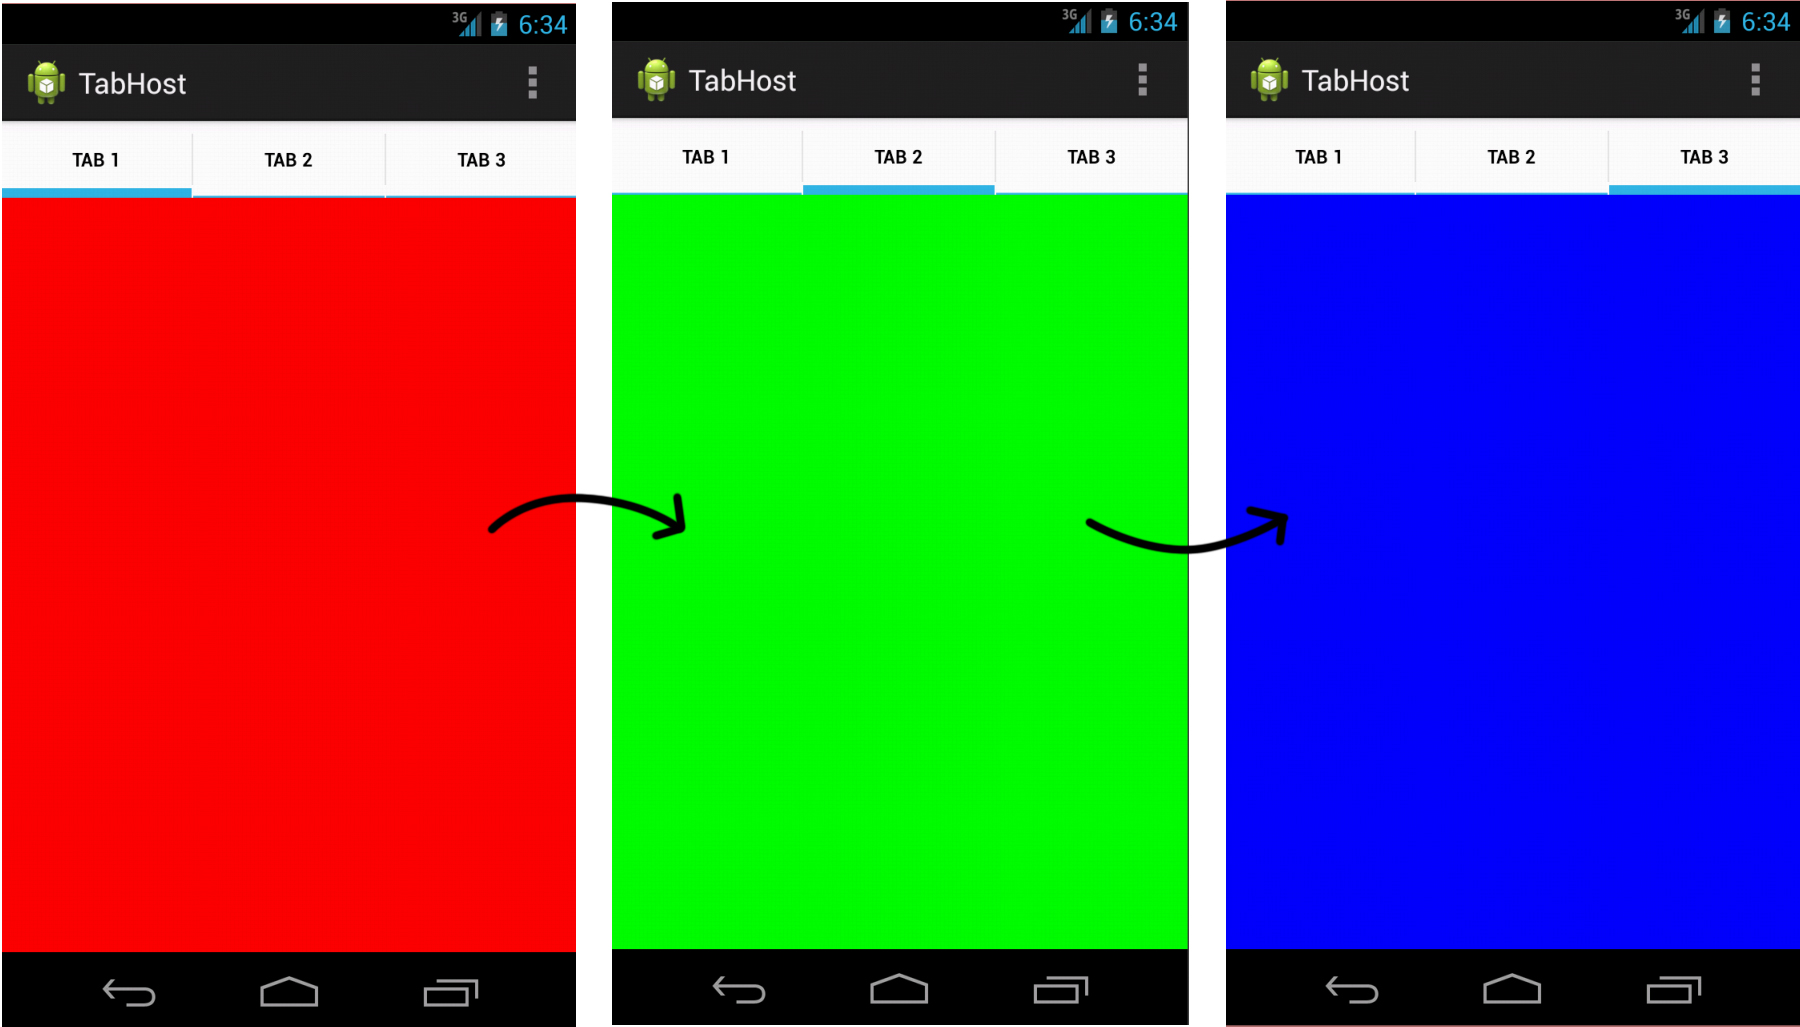
\includegraphics[width=1\textwidth]{figuras/design/tabs-rgb.jpg}
	  \caption{Figura mostrando as 3 abas criadas no exemplo}
	  \label{fig:e}
	\end{figure}
	
	
% SWIPE %
\section{Trocar de página com gesto de arrastar usando \texttt{ViewPager}}

	É possível trocar entre fragmentos usando o gesto de arrastar, isto é, arrastando a tela de um lado para o outro acionará a troca entre os fragmentos. 
	
	Primeiro iremos definir o \emph{layout} do \texttt{ViewPager}\footnote{\href{http://developer.android.com/reference/android/support/v4/view/ViewPager.html}{http://developer.android.com/reference/android/support/v4/view/ViewPager.html}}. Depois iremos definir o \texttt{PagerAdapter}\footnote{\href{http://developer.android.com/reference/android/support/v4/view/PagerAdapter.html}{http://developer.android.com/reference/android/support/v4/view/PagerAdapter.html}}. Por último precisamos definir a \emph{activity} que irá conter o visualizador de páginas. 
	
	\begin{listing}[H]
	\inputminted[linenos=true,fontsize=\small,frame=lines, framesep=2mm, tabsize=2,numbersep=5pt]{xml}{src/design/viewpager.xml}
	\caption{\emph{layout} do \texttt{ViewPager}}
	\end{listing}
	
	Agora defina uma nova classe chamada \texttt{PagerAdapter} que irá extender a classe \texttt{FragmentPagerAdapter}. Primeiro crie uma lista que irá conter os fragmentos, isto é, as páginas que serão exibidas. Ao extender essa classe precisamos implementar dois métodos: \texttt{getItem()} e \texttt{getCount()}. O método \texttt{getItem()}, na linha 10 do algoritmo \ref{code:pageadap}, deve retornar o item que será selecionado pelo parâmetro \texttt{position}. O método \texttt{getCount()}, na linha 15, deve retornar a quantidade de páginas. Depois crie o construtor como mostrado nas linhas 4-7. 

	\begin{listing}[H]
	\inputminted[linenos=true,fontsize=\small,frame=lines, framesep=2mm, tabsize=2,numbersep=5pt]{java}{src/design/pageradapter.java}
	\caption{Classe \texttt{PagerAdapter}}
	\label{code:pageadap}
	\end{listing}
	
	Por último devemos construir a \emph{activity} que irá conter o \texttt{PagerAdapter} e será reponsável por mostrar as páginas. Neste exemplo iremos reutilizar os fragmentos que fizemos na seção anterior quando trabalhamos com abas.
	
	\dica{Você pode importar as classes e os arquivos de \emph{layout}. No \emph{PackageExplorer} na IDE Eclipse, clique com o botão direito sobre a pasta que quer importar os arquivos, depois clique em \emph{Import} e selecione \emph{General -> File System}. Agora selecione o caminho da pasta que contém os arquivos no campo \emph{From directory}. Selecione os arquivos que deseja importar e clique em \emph{Finish}.
	
	Note que ao importar classes Java será necessário trocar o pacote a que a classe pertence.
	
	Outra opção é usar o \texttt{import} do java para importar as classes sem ter elas no pacote.}
	
	Essa \emph{activity}, como mostrada no algoritmo \ref{code:act-pager} abaixo, apenas precisa instanciar os fragmentos (linhas 10,11 e 12), criar e determinar o adaptador, linhas 14, 16 e 17.
	
	\begin{listing}[H]
	\inputminted[linenos=true,fontsize=\small,frame=lines, framesep=2mm, tabsize=2,numbersep=5pt]{java}{src/design/viewpager-activity.java}
	\caption{\emph{Activity} com \texttt{PagerAdapter}}
	\label{code:act-pager}
	\end{listing}

% SWIPEABLE TABS %
\section{Abas com gesto de arrastar}

	Ao juntar os dois conceitos, o de \emph{layout} com abas e o gesto de arrastar, podemos fazer o controle das abas arrastando a tela. Esse tipo de \emph{design} é comum em muitos aplicativos pela facilidade e rapidez com o que o usuário pode visualizar vários conteúdos. 
	Nesse exemplo iremos re-utilizar o código dos exemplos anteriores com algumas modificações. Serão reutilizadas classes: \texttt{TabInfo}, \texttt{TabFactory}, \texttt{PagerAdapter}, \texttt{Tab1Fragment}, \texttt{Tab2Fragment}, \texttt{Tab3Fragment}.
	
	Primeiro modificaremos o \emph{layout} das abas adicionando o \texttt{ViewPager} após \texttt{FrameLayout}. Note que esse é o mesmo \emph{layout} do algoritmo \ref{code:layout-tabhost}, por isso o algoritmo \ref{code:layout-viewpager} não está completo.
	
	\begin{listing}[H]
	\inputminted[linenos=true,fontsize=\small,frame=lines, framesep=2mm, tabsize=2,numbersep=5pt]{xml}{src/design/swipetabs-layout.xml}
	\caption{\emph{Layout} das abas com adição do \texttt{ViewPager}}
	\label{code:layout-viewpager}
	\end{listing}
	
	Agora iremos usar a classe \texttt{TabLayoutActivity} do exemplo anterior e fazer algumas alterações.  Nesse exemplo irei mudar o nome da classe para \texttt{SwipeTabActivity}. A primeira alteração é a adição de algumas variáveis para serem usadas na classe, adicione uma variável \texttt{PageAdapter} e uma \texttt{ViewPager}. Depois devemos alterar o método \texttt{onCreate()}, adicione uma chamada ao método \texttt{initialiseViewPager()}. A implementação é a mesma do método \texttt{onCreate()} do exemplo anterior com a adição da chamada ao método \texttt{setOnPageChangeListener()}. Devemos também implementar a interface \texttt{OnPageChangeListener}. No método \texttt{initialiseTabHost()} você precisa remover a linha \texttt{onTabChanged(''Tab1'');}.
	
	\begin{listing}[H]
	\inputminted[linenos=true,fontsize=\small,frame=lines, framesep=2mm, tabsize=2,numbersep=5pt]{java}{src/design/initialiseviewpager.java}
	\caption{Método \texttt{initialiseViewPager()}}
	\end{listing}
	
	Em seguida precisamos alterar o método \texttt{onTabChanged()}, não necessitamos mais fazer verificações já que o próprio \emph{design} irá limitar as falhas que poderiam ocorrer. Precisamos apenas determinar para o \texttt{ViewPager} o item atual. 
	
	\begin{listing}[H]
	\inputminted[linenos=true,fontsize=\small,frame=lines, framesep=2mm, tabsize=2,numbersep=5pt]{java}{src/design/ontabchanged-swipe.java}
	\caption{Método \texttt{onTabChanged()} alterado}
	\end{listing}
	
	Por fim, devemos implementar os métodos da interface \texttt{ViewPager.OnPageChangeListener}, somente o método \texttt{onPageSelected()} será usado, para selecionar a aba correspondente à pagina atual.
	
	\begin{listing}[H]
	\inputminted[linenos=true,fontsize=\small,frame=lines, framesep=2mm, tabsize=2,numbersep=5pt]{java}{src/design/vpinterface.java}
	\caption{Métodos da interface \texttt{ViewPager.OnPageChangeListener}}
	\end{listing}
		
	
	\dica{Pela dificuldade em acompanhar passo a passo a construção desse \emph{design}, é recomendável obter o código do projeto no repositório. Está sob o nome \emph{SwipeableTabs}.}


% NAV DRAWER
\section{Menu lateral \emph{(Navigation Drawer)}}

	O \emph{Sliding Menu} não é padrão no SDK do Android, mas é um tipo de \emph{design} que está sendo usado por muitos aplicativos famosos hoje em dia, tais como: Facebook, Linkedin, Foursquare, e outros. Consiste de um menu que fica escondido na lateral esquerda da tela e que pode ser acessado utilizando um gesto ''puxando'' o menu ou com um botão instalado na \emph{ActionBar}.
	
	Existe um projeto \emph{Open Source} que é bem conhecido, acessado por esse link no \href{https://github.com/jfeinstein10/SlidingMenu}{GitHub}\footnote{\href{https://github.com/jfeinstein10/SlidingMenu}{https://github.com/jfeinstein10/SlidingMenu}}.
	
	A imagem abaixo mostra o menu sendo usado no aplicativo do Facebook.
	
	\begin{figure}[H]
	  \centering
	  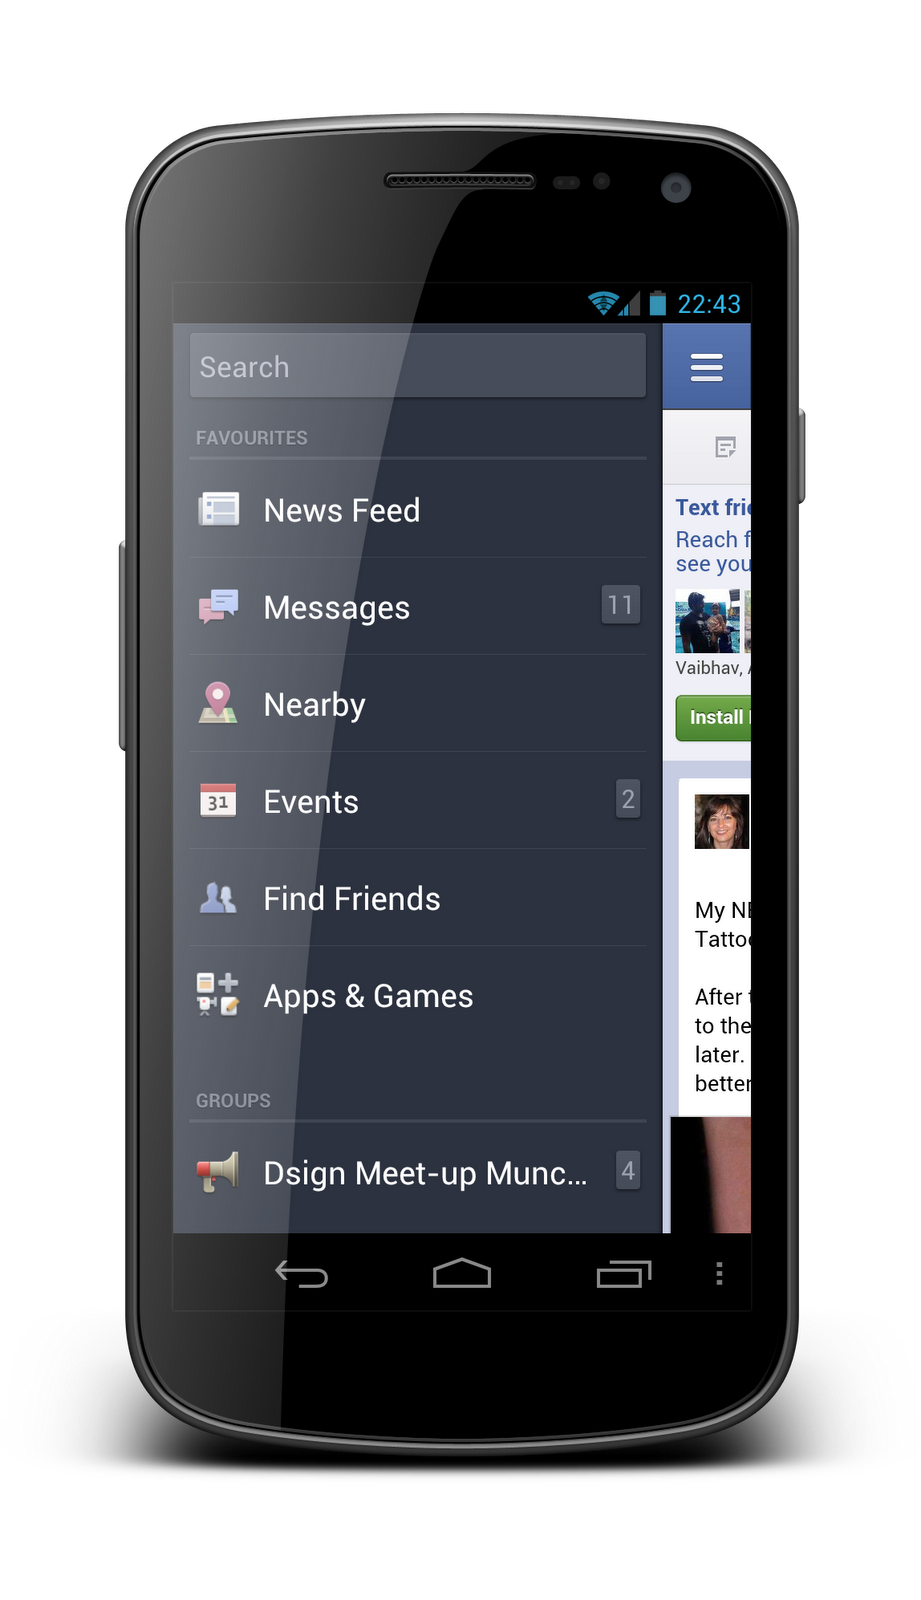
\includegraphics[width=.3\textwidth]{figuras/design/sidemenu.png}
	  \caption{Exemplo de \emph{Sliding Menu}}
	  \label{fig:e}
	\end{figure}
	
\section{\emph{ActionBar}}

	A \emph{ActionBar} é aquela barra presente em em todos os aplicativos que fizemos de exemplo até agora. Ela pode mostrar o nome da \emph{activity}, ícones, ações que podem ser acionadas, outras \emph{views} ou botões interativos. Também pode ser usada para navegar entre as \emph{actvities} do seu aplicativo.
	
	Dispositivos Android mais antigos possuem um botão físico chamado \emph{Option} que abre um menu na parte inferior do aplicativo. A \emph{ActionBar} é melhor que esse menu pois está claramente visível para o usuário, enquanto que o menu antigo era escondido e o usuário pode não reconhecer que as opções estão disponíveis.
	
	\begin{figure}[H]
	  \centering
	  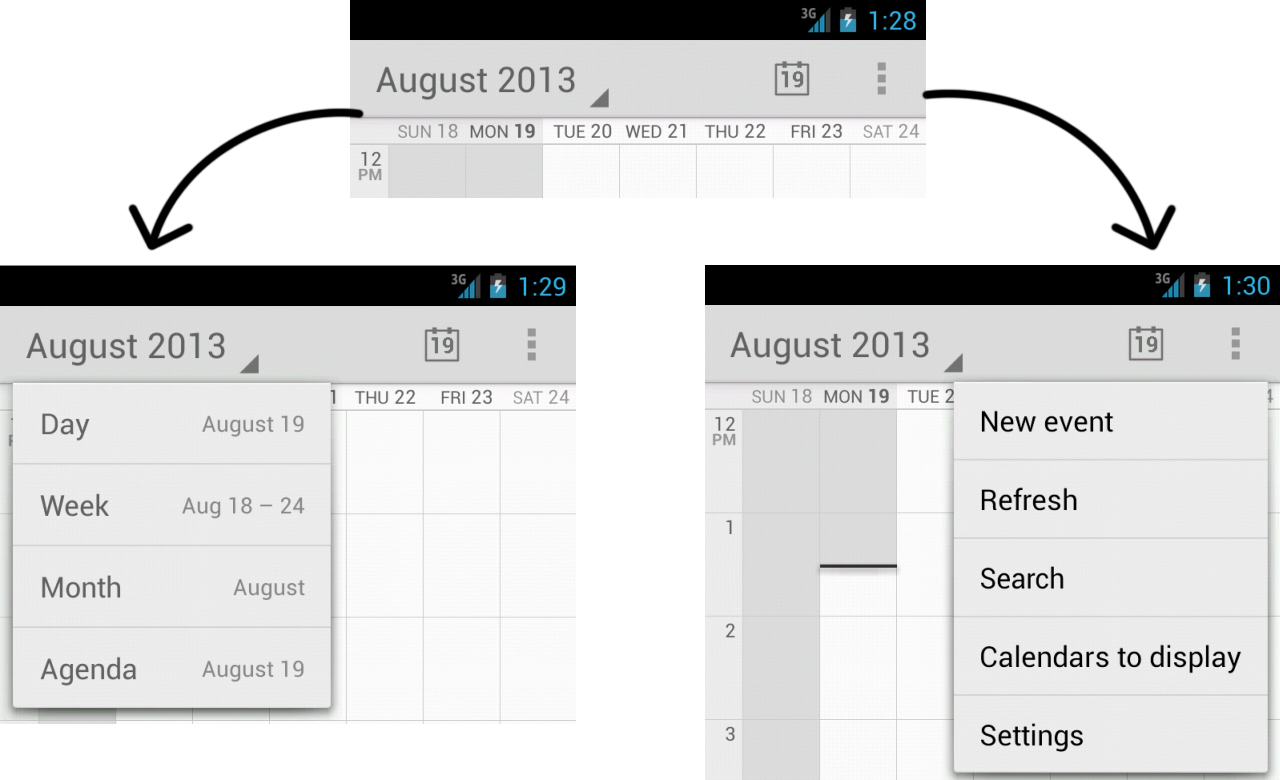
\includegraphics[width=.8\textwidth]{figuras/design/actionbar-ex.jpg}
	  \caption{Exemplo de \emph{ActionBar} no aplicativo Calendário}
	  \label{fig:e}
	\end{figure}
	
	A figura 5.18 mostra o uso da \emph{ActionBar} no aplicativo Calendário, padrão dos aparelhos Android mais atuais. É possivel observar três principais componentes. O primeiro é um menu \emph{drop-down} que permite ao usuário mudar o modo de vizualização do calendário. O segundo é um botão com o dia atual, 19, que ao ser pressionado faz com que o calendário posicione um cursor no dia e hora atuais. O terceiro é um outro menu \emph{drop-down} com algumas opções que podem ser interessantes ao usuário.
	
	\subsection{Implementando a \emph{ActionBar}}
	
		A \emph{activity} popula a \emph{ActionBar} em seu método \texttt{onCreateOptionsMenu()}. Entradas na \emph{ActionBar} são chamadas de ações (\emph{actions}). 
		
		As ações para a \emph{ActionBar} são definidas em arquivos XML posicionados na pasta \texttt{menu/}. O algoritmo abaixo mostra o menu padrão dos exemplos que construímos até agora. Ele só contem um item \emph{''Settings''} que está no \emph{dropdown} menu que pode ser acessado através da \emph{ActionBar}, à direita. O fato dele estar escondido se deve ao atributo \texttt{showAsAction} estar com valor \emph{never}, ao ser mudado para \emph{always} o acesso ao \emph{Settings} será diretamente através da \emph{ActionBar}. Existe também o valor \emph{ifRoom} que irá mostrar apenas se houver espaço disponível.
		
		\begin{listing}[H]
		\inputminted[linenos=true,fontsize=\small,frame=lines, framesep=2mm, tabsize=2,numbersep=5pt]{xml}{src/design/actionbar-menupadrao.xml}
		\caption{Menu padrão dos exemplos}
		\end{listing}

		\begin{listing}[H]
		\inputminted[linenos=true,fontsize=\small,frame=lines, framesep=2mm, tabsize=2,numbersep=5pt]{java}{src/design/oncreateoptionsmenu-padrao.java}
		\caption{Método padrão \texttt{onCreateOptionsMenu()}}
		\end{listing}
		
		Se uma ação e selecionada, o método \texttt{onOptionsItemSelected()} é chamado. Ele recebe a ação selecionada como parâmetro \texttt{MenuItem}. Baseando-se nessa informação você pode decidir o que fazer. Nesse exemplo iremos abrir uma nova \emph{activity} que seria a tela de configuração do aplicativo.
		
		No seu projeto, crie uma nova \emph{Activity} do tipo \emph{Settings Activity}. 
		
		\dica{Para criar uma nova \emph{activity}, clique com o botão direito sob o projeto selecione \emph{New -> Other} (ou pressione \emph{Ctrl+N}). Selecione \emph{Android Activity} e selecione o tipo desejado.}
		
		Agora você deve fazer com que o método \texttt{OnCreateOptionsMenu()} abra essa nova \emph{activity}.
		
		\begin{listing}[H]
		\inputminted[linenos=true,fontsize=\small,frame=lines, framesep=2mm, tabsize=2,numbersep=5pt]{java}{src/design/onoptionsitemselected.java}
		\caption{Método \texttt{OnOptionsItemSelected()}}
		\end{listing}

		Para melhorar nossa \emph{ActionBar} vamos adicionar um campo para pesquisa. Você pode adicionar \emph{views} em sua \emph{ActionBar}. Para isso você deve usar o método \texttt{setCustomView()}  da classe \texttt{ActionBar} e passar uma \emph{view} como parâmetro. Você também precisa ativar a exibição de \emph{views} com o método \texttt{setDisplayOptions()} e passar a \emph{flag} \texttt{ActionBar.DISPLAY\_SHOW\_CUSTOM}.
		
		Primeiro vamos adicionar um ícone de busca na nossa \emph{ActionBar}, voltando ao arquivo do \emph{layout} da \emph{ActionBar}, adicione um novo item acima do primeiro como mostrado no algoritmo abaixo.
		
		\begin{listing}[H]
		\inputminted[linenos=true,fontsize=\small,frame=lines, framesep=2mm, tabsize=2,numbersep=5pt]{xml}{src/design/newitem.xml}
		\caption{Adicionando novo item na \emph{ActionBar}}
		\end{listing}
		
		Observe o atributo \texttt{android:icon}, estamos obtendo um \emph{drawable} que já existe no sistema Android, e se chama \emph{ic\_menu\_search}. Esse é o ícone da busca, a lupa. Depois vamos adicionar uma ação a ser executada quando esse ícone for clicado. Iremos criar nesse exemplo, uma caixa de texto de forma programática, isto é, em vez de defini-la no XML iremos cria-la com código na \emph{Activity}. 
		
		No método \texttt{onCreate()} você precisa configurar a \emph{ActionBar} para mostrar \emph{views}. Use o método \texttt{getActionBar()} para obter uma referência da \emph{ActionBar} e \texttt{setDisplayOptions()} para configura-la. Depois, no método \texttt{onOptionsItemSelected()} você vai programar a ação do novo botão. Inicialmente cria-se uma nova \emph{view} do tipo \texttt{EditText}, colocamos algumas configurações e a adicionamos na \emph{ActionBar}. Por não termos uma busca devidamente implementada, vamos mostrar um \texttt{Toast} com o conteúdo da busca, a fim de demonstração.
		
		\begin{listing}[H]
		\inputminted[linenos=true,fontsize=\small,frame=lines, framesep=2mm, tabsize=2,numbersep=5pt]{java}{src/design/actionbar-oncreate.java}
		\caption{Configurando \emph{ActionBar} no método \texttt{onCreate()}}
		\end{listing}
		
		No algoritmo \ref{code:actionbar-seach}, abaixo, criamos um \texttt{EditText} e o configuramos caso o botão com o ícone de busca seja pressionado. Na linha 5-6 criamos um \texttt{LayoutParams} que configura o tamanho da \emph{view}. Na linha 8 o método \texttt{EditText.setImeOptions()} é responsável por configurar o teclado para uma busca, junto com a linha 9 que diz para o \texttt{EditText} que a entrada será texto, essa combinação faz com que o teclado mostre o ícone da lupa no lugar da tecla \emph{Enter}. A linha 10 configura a cor do texto para branca. Adicionamos a \emph{view} na \emph{ActionBar} com o método \texttt{ActionBar.setCustomView()} e passamos como parâmetro a \emph{view} criada e os parâmetros de \emph{layout} criados. O método \texttt{EditText.requestFocus()} faz com que o foco seja dado à nova caixa de texto, para que possamos edita-la. Precisamos ainda fazer com que o teclado abra para que possamos editar a caixa de texto, é isso que as linhas 13-14 e 15 estão fazendo. O método \texttt{getSystemService()} obtem a referência de um serviço do Android, e nesse caso estamos pedindo pelo serviço de método de entrada, o teclado. O método \texttt{InputMethodManager.showSoftInput()} abre o \emph{Soft Input}, ou seja, o teclado virtual para edição da \emph{view}. 
		
		Finalmente fazemos com que ao botão de busca no teclado ser clicado, um \texttt{Toast} mostre para o usuário o conteúdo da caixa de texto. É isso que a interface \texttt{onEditorActionListener} faz com o método \texttt{onEditorAction()}.
		
		A intenção desse exemplo é mostrar como você pode adicionar novas \emph{views} na \emph{ActionBar} de forma dinâmica.
		 
		\begin{listing}[H]
		\inputminted[linenos=true,fontsize=\small,frame=lines, framesep=2mm, tabsize=2,numbersep=5pt]{java}{src/design/actionbar-acao.java}
		\caption{Criando a caixa de busca na \emph{ActionBar}}
		\label{code:actionbar-seach}
		\end{listing}
		
		
	\begin{figure}[H]
	  \centering
	  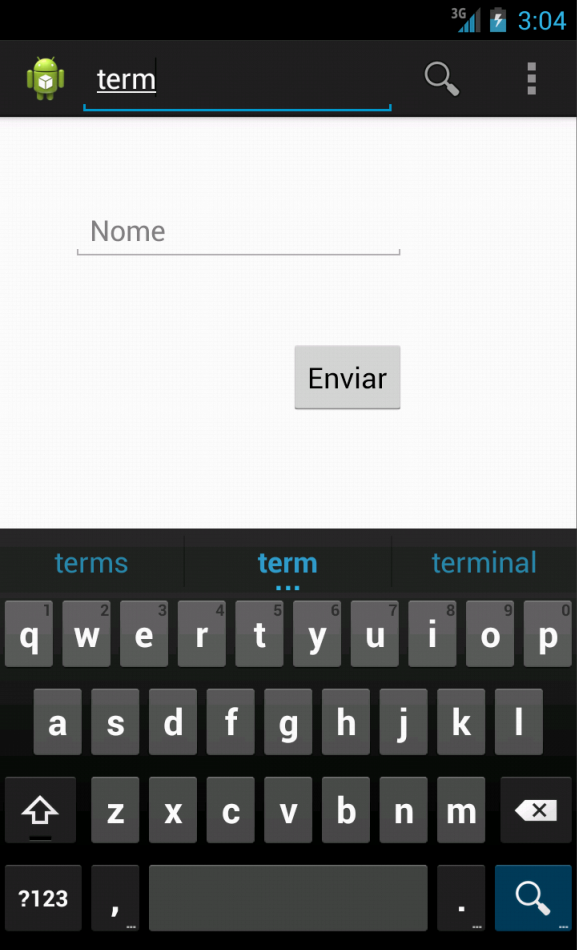
\includegraphics[width=.3\textwidth]{figuras/design/actionbar-search.png}
	  \caption{Exemplo de busca na \emph{ActionBar}}
	  \label{fig:e}
	\end{figure}


\chapter{Comunicação}

	Agora iremos explorar as funcionalidades de comunicação dos aparelhos Android como acesso a \emph{Internet} no caso de \emph{Tables} e \emph{Smartphones} e envio de SMS e chamadas de voz com os os \emph{Smartphones}. 

\section{\emph{Internet}}

	Antes de iniciar sua aplicação que faz acesso à \emph{Internet}, devemos dar permissão ao aplicativo através do arquivo de \emph{Manifest}. Logo antes da tag \texttt{uses-sdk} você deve adicionar a tag \texttt{uses-permission}, como mostrado abaixo:

		\begin{listing}[H]
		\inputminted[linenos=true,fontsize=\small,frame=lines, framesep=2mm, tabsize=2,numbersep=5pt]{xml}{src/api/comm/permission-internet.xml}
		\caption{Atribuindo permissão de acesso à \emph{Internet} no \emph{Manifest}}
		\label{code:permission-internet}
		\end{listing}

		Nesta seção, veremos como se faz requisições HTTP para obter páginas HTML, saídas de um \emph{script server-side} como PHP ou ASP.NET e \emph{parsing} de respostas JSON ou XML.		 

		\subsection{HTTP GET}

		Para fazer uma requisição HTTP GET usaremos as classes da biblioteca \emph{Apache}, tais como \emph{HttpClient}, \emph{HttpGet} e \emph{HttpResponse}. Primeiros crie uma classe que iremos chamar de \texttt{RequestTask} e ela deve extender a classe \texttt{AsyncTask}\footnote{\href{http://developer.android.com/reference/android/os/AsyncTask.html}{http://developer.android.com/reference/android/os/AsyncTask.html}}, ela vai permitir que façamos a requisição na \emph{thread} da interface do usuário sem precisar criar e manipular uma \emph{thread} diferente.

		\begin{listing}[H]
		\inputminted[linenos=true,fontsize=\small,frame=lines, framesep=2mm, tabsize=2,numbersep=5pt]{java}{src/api/comm/asynctask.java}
		\caption{Classe \texttt{RequestTask}}
		\label{code:requesttask}
		\end{listing}

		O método \texttt{doInBackground()} é o responsável por realizar a operação sem o usuário perceber. Existem outros dois métodos da classe \texttt{AsyncTask} que podem ser utilizados: \texttt{onProgressUpdate()}, caso queira mostrar o progresso de um \emph{download} para o usuário e \texttt{onPostExecute()} para executar alguma ação após o termino do \emph{download}.

		Observe o algoritmo \ref{code:requesttask}, na linha 5-7 criamos um novo \texttt{HttpClient}, \texttt{HttpResponse} e uma \emph{string} para armazenar a resposta do servidor. Depois, envolto por um bloco \texttt{try-catch} temos uma chamada ao método \texttt{HttpClient.execute()} e é passado para ele um novo \texttt{HttpGet} com o parâmetro \texttt{uri[0]}, \texttt{uri} é um dos parâmetros do método e contém uma URI\footnote{\href{http://developer.android.com/reference/java/net/URI.html}{http://developer.android.com/reference/java/net/URI.html}} que identifica o destino da requisição.

		Na linha 11 foi criado um novo \texttt{StatusLine}\footnote{\href{http://developer.android.com/reference/org/apache/http/StatusLine.html}{http://developer.android.com/reference/org/apache/http/StatusLine.html}} para guardar a resposta da requisição HTTP que obtemos com o método \texttt{HttpResponse.getStatusLine()}. Depois comparamos o código do \emph{status} com \texttt{HttpStatus.SC\_OK} (equivalente ao código 200), o \emph{status} \texttt{OK} significa que a requisição e a resposta ocorreram como esperado e temos a resposta correta vindo do servidor. 

		Em seguita criamos um novo \texttt{ByteArrayOutputStream} que é responsável por guardar a resposta do servidor na chamada ao método \texttt{HttpResponse.getEntity().writeTo()}. Por último convertemos o \emph{byte stream} em uma string usando o método \texttt{toString()} e a retornamos.

		Agora precisamos de uma \emph{Activity} para mostrar a resposta, nesse exemplo obteremos o código HTML da página do DC UFSCar: \href{http://www.dc.ufscar.br}{http://www.dc.ufscar.br}. Mostraremos o código HTML como uma página \emph{Web} usando o \texttt{WebView}.

		\begin{listing}[H]
		\inputminted[linenos=true,fontsize=\small,frame=lines, framesep=2mm, tabsize=2,numbersep=5pt]{java}{src/api/comm/httpget.java}
		\caption{Classe \texttt{RequestTask}}
		\label{code:requestactivity}
		\end{listing}		

		Primeiro criamos uma nova variável \texttt{task} do tipo \texttt{AsyncTask} nos moldes da classe que criamos, dentro de um bloco \texttt{try-catch} criamos uma nova \texttt{URI} e atribuímos a ela o endereço da página do DC UFSCar. Em seguida iniciamos a variável \texttt{task} criando uma nova \texttt{RequestTask} e chamamos o método \texttt{execute()}, que ao ser chamado irá executar o método \texttt{doInBackground()}. 
		
		Por fim, criamos uma nova \texttt{WebView}\footnote{\href{http://developer.android.com/reference/android/webkit/WebView.html}{http://developer.android.com/reference/android/webkit/WebView.html}} e carregamos o conteúdo da \emph{string} \texttt{response} nela usando o método \texttt{WebView.loadData()}. A página é mostrada sem estilo pois não estamos puxando as folhas de estilo junto, somente o código HTML.
		
		 \dica{Usamos a \texttt{WebView} para mostrar o código HTML como página apenas para demonstração. Caso queira carregar uma página corretamente deve fornecer a \emph{URL} da página diretamente para a \texttt{WebView}.}

		\subsection{HTTP POST}
		Diferentemente do \emph{GET}, onde os parâmetros para o servidor vão codificados na \emph{URL}, no \emph{POST} os parâmetros vão codificados no final do cabeçalho HTTP. Para enviar uma requisição do tipo \emph{POST}, usaremos a classe \texttt{HttpPost}. O algoritmo abaixo é reaproveitado da classe \texttt{RequestTask} e do método \texttt{doInBackgrond()}, onde mudaremos apenas algumas linhas. Agora estaremos enviando a requisição para essa página: \href{http://httpbin.org/post}{http://httpbin.org/post}, ela só aceita requisições do tipo \emph{POST}, se tentar com \emph{GET} irá receber uma mensagem de erro.

		\begin{listing}[H]
		\inputminted[linenos=true,fontsize=\small,frame=lines, framesep=2mm, tabsize=2,numbersep=5pt]{java}{src/api/comm/httppost.java}
		\caption{Modificando o método para requsições \emph{POST}}
		\label{code:httppost}
		\end{listing} 

		Criamos um novo \texttt{HttpPost}\footnote{\href{http://developer.android.com/reference/org/apache/http/client/methods/HttpPost.html}{http://developer.android.com/reference/org/apache/http/client/methods/HttpPost.html}} passando a \texttt{URI} como parâmetro. Criamos uma lista de tuplas chave-valor que representa a variável e seu valor no cabeçalho HTTP e adicionamos dois valores. Em seguida chamamos o método \texttt{HttpPost.setEntity()} e passamos um objeto do tipo \texttt{UrlEncodedFormEntity}\footnote{\href{http://developer.android.com/reference/org/apache/http/client/entity/UrlEncodedFormEntity.html}{http://developer.android.com/reference/org/apache/http/client/entity/UrlEncodedFormEntity.html}} que recebe a lista como parâmetro, esse objeto irá codificar a lista em variáveis aceitas pelo padrão de uma requisição \emph{POST}.

		Por final, executamos a requisição como feito anteriormente. O resto do código é igual.

 		Note que se colocar a resposta dessa requisição em uma \texttt{WebView} ou \texttt{TextView} irá observar que está codificado no formato JSON\footnote{O que é JSON: \href{http://www.json.org/}{http://www.json.org/}}. 

		\subsection{Decodificando JSON}
		
		Vamos obter dados do objeto JSON retornado pelo exemplo anterior. Se você observar a \emph{string} na tela, irá perceber os dados que foram enviado via \emph{POST} dentro de um objeto JSON chamado \emph{form}. Queremos obter esses dados, para isso precisamos criar uma classe que será responsável por obter especificamente esses dados do \emph{form}.
		
		\dica{Em JSON, \{ representa um objeto JSON e [ representa um \emph{array} dentro de um objeto JSON}

		Crie uma classe \texttt{JSONParser}, como mostrado abaixo.
		
		\begin{listing}[H]
		\inputminted[linenos=true,fontsize=\small,frame=lines, framesep=2mm, tabsize=2,numbersep=5pt]{java}{src/api/comm/jsonparser.java}
		\caption{Classe \texttt{JSONParser}}
		\label{code:jsonparser}
		\end{listing} 

		Para obter dados do \emph{form}, criamos um método \texttt{getFormData()}. Primeiro obtemos o objeto JSON dado pela \emph{string} retornada pela requisição \emph{POST} do exemplo anterior ao criar um novo \texttt{JSONObject} e passando a \emph{string} como parâmetro. Em seguida queremos obter outro objeto JSON, aquele cujo nome é \emph{form}, para isso chamamos o método \texttt{JSONObject.getJSONObject()} passando o nome do objeto junto. Após obter o objeto desejado, usamos o método \texttt{JSONObject.getString()} e passamos o nome do valor para obter o valor. Então ao passar \emph{"testing"} e \emph{"user"} esperamos como retorno \emph{POST} e \emph{You}, respectivamente. 

		\subsection{Codificando JSON}

		Podemos também codificar objetos JSON, e é simples. Basta criar um \texttt{JSONObject} ou \texttt{JSONArray} e usar o método \texttt{toString()}. Por exemplo:
	
		\begin{listing}[H]
		\inputminted[linenos=true,fontsize=\small,frame=lines, framesep=2mm, tabsize=2,numbersep=5pt]{java}{src/api/comm/writejson.java}
		\caption{Criando JSON}
		\label{code:jsonparser}
		\end{listing} 


	\section{Telefone}
		
		É possível fazer uma chamada telefônica, porém você terá que usar o discador padrão do Android uma vez que ele não provê uma API pública para fazer chamadas diretamente pelo seu aplicativo. A única forma é através do interemediador \texttt{ACTION\_CALL}. O Exemplo abaixo mostra como fazer uma chamada usando esse intermediador.

		\begin{listing}[H]
		\inputminted[linenos=true,fontsize=\small,frame=lines, framesep=2mm, tabsize=2,numbersep=5pt]{java}{src/api/comm/phonecall.java}
		\caption{Fazendo uma chamada telefônica}
		\label{code:phonecall}
		\end{listing} 

		Para esse exemplo, foi criado uma caixa de texto e um botão, o número de telefone é colocado na caixa de texto e o botão \emph{Call} inicia a \emph{activity} responsável por realizar a chamada. Observe que é necessário fazer um \emph{parse} do número de telefone para uma \emph{URI} com formato \texttt{tel:0123456789}. Cria-se uma \texttt{Intent} para o \texttt{ACTION\_CALL}, coloca-se os dados na \texttt{Intent} e chama o método \texttt{startActivity()} para fazer a chamada telefônica. É preciso dar permissão ao aplicativo para fazer chamadas adicionando essa linha ao \emph{Manifest}.
	
		\begin{listing}[H]
		\inputminted[linenos=true,fontsize=\small,frame=lines, framesep=2mm, tabsize=2,numbersep=5pt]{xml}{src/api/comm/phonecall-perm.xml}
		\caption{Permissão para fazer chamadas telefônicas}
		\label{code:phonecall-perm}
		\end{listing} 		

		Usando a classe \texttt{TelephonyManager}\footnote{\href{http://developer.android.com/reference/android/telephony/TelephonyManager.html}{http://developer.android.com/reference/android/telephony/TelephonyManager.html}}, no entanto, o Android nos dá a possibilidade obter dados do \emph{Sim Card} e também um \emph{listener} para saber o status atual do telefone, se ele está fazendo uma ligação ou não.

		Você pode usar os métodos \texttt{getDeviceId()} para obter o número IMEI do aparelho, \texttt{getSimSerialNumber()} para obter o número de série do \emph{Sim Card}, \texttt{isNetworkRoaming()} para saber se está em modo \emph{roaming}, etc.

	\section{\emph{Short Message Service (SMS)}}

		O Android provê uma API pública para mandar mensagens SMS, através da classe \texttt{SMSManager}\footnote{\href{http://developer.android.com/reference/android/telephony/SmsManager.html}{http://developer.android.com/reference/android/telephony/SmsManager.html}}. Assim como fazer ligações, enviar SMS também precisa configurar a permissão no \emph{Manifest}.

		\begin{listing}[H]
		\inputminted[linenos=true,fontsize=\small,frame=lines, framesep=2mm, tabsize=2,numbersep=5pt]{xml}{src/api/comm/sms-perm.xml}
		\caption{Permissão para enviar mensagens SMS}
		\label{code:sms-perm}
		\end{listing} 	

		Agora vamos criar um aplicativo simples que chama a classe \texttt{SMSManager} para enviar uma mensagem para um número de telefone. Teremos duas \texttt{EditText} \emph{views} para abrigar a mensagem e o número, e um botão para enviar. Inicialmente crie um método \texttt{sendSMS()}.

		\begin{listing}[H]
		\inputminted[linenos=true,fontsize=\small,frame=lines, framesep=2mm, tabsize=2,numbersep=5pt]{java}{src/api/comm/sendsms.java}
		\caption{Método \texttt{sendSMS()}}
		\label{code:sendsms}
		\end{listing} 	
	
		Dentro de um bloco \texttt{try-catch} crie um novo \texttt{SMSManager} como mostrado na linha 3 do algoritmo \ref{code:sendsms}, use o método \texttt{SmsManager.sendTextMessage()} para enviar uma mensagem. O primeiro parâmetro é o número de telefone para qual a mensagem será enviada, o segundo é o telefone de origem, colocando \texttt{null} o valor será o número do próprio aparelho ou serviço, o terceiro parâmetro é o texto da mensagem.
		
		Completanto, com um algoritmo simples para chamar o método quando o botão for pressionado.

		\begin{listing}[H]
		\inputminted[linenos=true,fontsize=\small,frame=lines, framesep=2mm, tabsize=2,numbersep=5pt]{java}{src/api/comm/sendsms-oncreate.java}
		\caption{Chamando método \texttt{sendSMS()}}
		\label{code:sendsms}
		\end{listing} 	

\chapter{Armazenamento}

	O Android provê algumas opções para que você possa salvar dados persistentes de sua aplicação. A escolha da opção de armazenamento vai depender das necessidades da sua aplicação, isto é, se os dados vão ser visíveis somente pela aplicação ou se o usuário terá acesso a eles, quanto de espaço será necessario, que tipo de dados você pretende salvar.
	As opções são: 
	\bi
		\item \emph{Shared Preferences}: Usada principalmente para salvar preferências do usuário, esse método guarda primitivas em duplas chave-valor;
		\item Armazenamento Interno: Salva dados privados na memória do dispositivo;
		\item Armazenamento Externo: Salva dados públicos na memória externa compartilhada;
		\item Bancos de Dado \emph{SQLite}: Salva dados estruturados em um banco de dados privado.
		\item Conexão com a rede: Salva dados na \emph{web} em seu próprio servidor na rede.
	\ei
			
	\section{\emph{Shared Preferences:}}
		
		A classe \texttt{SharedPreferences}\footnote{\href{http://developer.android.com/reference/android/content/SharedPreferences.html}{http://developer.android.com/reference/android/content/SharedPreferences.html}} fornece um framework que te permite salvar e recuperar dados primitivos persistentes no formato chave-valor. Você pode salvar qualquer tipo de dado primitivo: \emph{booleans}, \emph{floats}, inteiros, \emph{longs} e \emph{strings}.
 
		Você pode usar essa classe para armazenar dados durante o ciclo de vida de uma \emph{activity}. Isto é, antes da \emph{activity} ser destruída na função \texttt{onDestroy()}, os dados podem ser salvos durante a execução de \texttt{onStop()} e recuperados na execução de \texttt{onCreate()}.

		Para usar a \texttt{SharedPreferences} na sua aplicação você deve chamar \texttt{getSharedPreferences()} se precisar de vários arquivos de preferencias que serão identificados pelo nome ou \texttt{getPreferences()} se precisar de apenas um arquivo para sua \emph{activity}, esse não necessita de nome pois será único para a \emph{activity}. Em seguida para escrever valores você deve chamar o método \texttt{edit()} para obter um \texttt{SharedPreferences.Editor}, e usar os métodos como \texttt{putString()} para adicionar novos valores. Por último \texttt{commit()} deve ser chamado para salvar os valores. Para ler os valores, você deve chamar métodos como \texttt{getBoolean()} ou \texttt{getString()}.

		O exemplo abaixo salva os dados de uma caixa de texto, uma barra de progresso e uma chave em uma \texttt{SharedPreferences} e depois os lê quando o aplicativo é aberto novamente.

		\begin{listing}[H]
		\inputminted[linenos=true,fontsize=\small,frame=lines, framesep=2mm, tabsize=2,numbersep=5pt]{java}{src/api/storage/sharedpref.java}
		\caption{Utilizando \texttt{SharedPreferences} para salvar dados primitivos}
		\label{code:sharedpref}
		\end{listing} 	
		
		Observe no algoritmo \ref{code:sharedpref} a utilização da classe \texttt{SharedPreferences}, no método \texttt{onStop()} chamamos o método \texttt{getPreferences(MODE\_PRIVATE)} para obter uma instância da classe no modo privado, isto é, os dados somente são acessíveis por esta \emph{activity} deste aplicativo. Na linha 30 obtemos o \texttt{SharedPreferences.Editor} ao chamar o método \texttt{SharedPreferences.edit()}.
		
		O \texttt{Editor} é usado então para adicionar os valores que obtemos das \emph{views}. Na linha 32 usamos \texttt{putString()} para guardar o conteúdo da caixa de texto,
\texttt{putInt()} para guardar a posição da \texttt{SeekBar} e \texttt{putBoolean()} para guardar o estado da chave. Finalmente invocamos \texttt{commit()} para salvar os dados.

		No método \texttt{onCreate()} usamos os métodos \texttt{get} para obter os dados que foram salvos. Esses métodos requerem a passagem de um valor \emph{default} para quando não há dados previamente salvos. Observe então nas linhas 16-18 que para a caixa de texto usamos uma \emph{string} vazia, para a \texttt{SeekBar} o valor 0 e a chave desligada.


		\section{Armazenamento interno}

		Você pode salvar arquivos diretamente na memória interna do dispositivo. Por padrão os arquivos salvos no armazenamento interno são privados a seu aplicativo e não podem ser acessados por outros aplicativos. 

		Para criar um novo arquivo você deve invocar o método \texttt{openFileOutput()} passando o nome do arquivo e o modo de operação. Esse método irá retornar um \texttt{FileOutputStream}. Você poderá escrever nesse arquivo chamando o método \texttt{FileOutputStream.write()} e \texttt{FileOutputStream.close()} para fechar o arquivo.

		Para exemplificar, faremos um aplicativo do tipo bloco de notas. Será composto de dois botões, um para abrir um arquivo e outro para salvar um arquivo, e uma caixa de texto para escrever. Tudo será feito no método \texttt{onCreate()}, primeiro  usamos \texttt{findViewById()} para obter as \emph{views}. O botão de salvar irá abrir um dialogo perguntando o nome do arquivo, e o botão de abrir mostrará um dialogo permitindo ao usuário escolher dentre os arquivos já salvos anteriormente.

		No código abaixo criamos o \emph{listener} do botão de salvar, dentro dele criamos um dialogo e precisamos de um \emph{listener} para confirmar e um para cancelar.

		\begin{listing}[H]
		\inputminted[linenos=true,fontsize=\small,frame=lines, framesep=2mm, tabsize=2,numbersep=5pt]{java}{src/api/storage/internal1.java}
		\caption{Passos iniciais do \emph{listener}, criando um dialogo.}
		\label{code:internal1}
		\end{listing} 	

		Com o \texttt{AlertDialog.Builder} começamos a construir um novo diálogo. Usamos o \texttt{LayoutInflater} para carregar o \emph{layout} com uma \texttt{EditText}.
		Chamamos \texttt{setPositivoButton()} para criar um \emph{listener} que irá salvar o arquivo quando o botão for clicado.

		\begin{listing}[H]
		\inputminted[linenos=true,fontsize=\small,frame=lines, framesep=2mm, tabsize=2,numbersep=5pt]{java}{src/api/storage/internal2.java}
		\caption{Salvando um arquivo e mostrando um \texttt{Toast}}
		\label{code:internal2}
		\end{listing} 	

		Vamos analisar o algoritmo \ref{code:internal2}. Na linha 5 queremos a referência ao \texttt{EditText} contido no diálogo, para isso precisamos usar a variável \texttt{fnameEntry} criada ao chamar o método \texttt{LayoutInflater.inflate()}. Depois, na linha 7-8 certificamos que o nome do arquivo não será vazio (se for vazio, o arquivo não é salvo), para isso atribuimos o nome \emph{untitled} a ele. Obtemos também o texto escrito na caixa de texto da \emph{activity} na linha 9.

		Agora que já temos o nome e os dados do arquivo, precisamos efetivamente salvá-lo no armazenamento interno. Com o método \texttt{openFileOutput()} teremos um \texttt{FileOutputStream} que servirá para escrever os dados no arquivo. Isso é feito nas linhas 13-14 com o método \texttt{write()} e em seguida o método \texttt{close()}.
		Para certificar ao usuário que o arquivo foi salvo, mostramos um \texttt{Toast} com a mensagem que o arquivo foi salvo.

		Se o usuário clicar em \emph{cancel} no diálogo, precisamos fechá-lo, basta invocar \texttt{dialog.close()} no \emph{listener}.

		\begin{listing}[H]
		\inputminted[linenos=true,fontsize=\small,frame=lines, framesep=2mm, tabsize=2,numbersep=5pt]{java}{src/api/storage/internal3.java}
		\caption{Fechando o dialogo ao clicar em \emph{close}}
		\label{code:internal3}
		\end{listing} 	

		Depois chame \texttt{builder.create().show()} no \texttt{listener} do botão \emph{Save} para mostrar o diálogo.
 
		Para o botão \emph{Open} iremos mostrar um dialogo com os nomes dos arquivos salvos anteriormente, quando um desses for clicado o arquivo se abrirá preenchendo a caixa de texto.

		\begin{listing}[H]
		\inputminted[linenos=true,fontsize=\small,frame=lines, framesep=2mm, tabsize=2,numbersep=5pt]{java}{src/api/storage/internal4.java}
		\caption{Criando um diálogo com os arquivos salvos}
		\label{code:internal4}
		\end{listing} 	
	
		Dessa vez usamos o método \texttt{builder.setItems()} para construir uma lista no diálogo. O método \texttt{fileList()} retorna um \texttt{array} de nomes de arquivo que foram armazenados internalmente no aplicativo. 

		\begin{listing}[H]
		\inputminted[linenos=true,fontsize=\small,frame=lines, framesep=2mm, tabsize=2,numbersep=5pt]{java}{src/api/storage/internal5.java}
		\caption{Criando um diálogo com os arquivos salvos}
		\label{code:internal5}
		\end{listing} 	
		
		Na linha 7 do algoritmo \ref{code:internal5} queremos obter a referência do arquivo selecionado. Chamando o método \texttt{getFilesDir()} nos é fornecido o diretório contendo os arquivos, com \texttt{listFiles()} temos um \emph{array} de \texttt{Files} e o selecionamos com a variável \texttt{which}, que é a posição clicada na lista do diálogo. Para ler os dados desse arquivo, usamos a classe \texttt{BufferedReader} e guardamos as linhas sendo lidas em um objeto do tipo \texttt{StringBuilder}. Nas linhas 13-16 lemos cada linha do arquivo em um loop \emph{while} e usamos o método \texttt{append()} duas vezes, uma para adicionar a linha lida na \emph{string} e outra para adicionar o separador de linha (comummente \textbackslash n). Ao fim invocamos \texttt{close()} para fechar o \texttt{BufferedReader}. E colocamos o texto lido de volta na caixa de texto.

 
		
			 
\end{singlespace}



%%%%%%%%%%%%%%%%%%%%%%%%%%%%%%%%%%%%%%%%%%%%%%%%%%%%%%%%%%%%%%%%%%%%%%%%%%%%%%%%

\singlespace
\selectlanguage{brazil}
\clearpage
\thispagestyle{empty}
\phantomsection
\doublespace


\appendix
\addtocontents{toc}{\protect\setcounter{tocdepth}{0}} % as seções do apêndice não aparecem do sumário com este comando...
%%%%%%%%%%%%%%%%%%%%%%%%%%%%%%%%%%%%%%%%%%%%%%%%%%%%%%%%%%%%%%%%%%%%%%%%%%%%%%%%
\ape{apen}{Especificação blá, blá, blá}

Isto é um apêndice...

%%%%%%%%%%%%%%%%%%%%%%%%%%%%%%%%%%%%%%%%%%%%%%%%%%%%%%%%%%%%%%%%%%%%%%%%%%%%%%%%
\addtocontents{toc}{\protect\setcounter{tocdepth}{1}}

\end{document}
